\documentclass[openany]{book}

\usepackage[italian]{babel}

\usepackage[a4paper,top=2cm,bottom=2cm,left=2cm,right=2cm,marginparwidth=1.75cm]{geometry}

\usepackage{showframe}

\usepackage{amsmath, amssymb}
\usepackage{graphicx}
\usepackage[hidelinks]{hyperref}

% Define colors for name-verb analysis and legend
% https://www.overleaf.com/learn/latex/Using_colors_in_LaTeX
\usepackage{soul}
\usepackage[dvipsnames]{xcolor}
\colorlet{ColorClass}{Cyan}
\colorlet{ColorAttr}{BurntOrange}
\colorlet{ColorFunc}{GreenYellow}
\colorlet{ColorActor}{Red}
\colorlet{ColorClassActor}{Thistle}
\newcommand{\Class}[1]{\sethlcolor{ColorClass}\hl{#1}}
\newcommand{\Attr}[1]{\sethlcolor{ColorAttr}\hl{#1}}
\newcommand{\Func}[1]{\sethlcolor{ColorFunc}\hl{#1}}
\newcommand{\Actor}[1]{\sethlcolor{ColorActor}\hl{#1}}
\newcommand{\ClassActor}[1]{\sethlcolor{ColorClassActor}\hl{#1}}

% requisiti
\newcommand{\Req}[2]{\textsc{#1$_{#2}$}}

\usepackage{tabularray}
\UseTblrLibrary{varwidth}
\usepackage{enumitem}
\usepackage{eurosym}
\usepackage{minted}

\usepackage{tikz}
\usetikzlibrary{shapes.geometric, arrows, positioning, fit}

% Tabella per gli scenari
\NewTblrEnviron{scenery}
\SetTblrInner[scenery]{
	hlines, vlines,
	% rowsep=1.5pt,
	row{1} = {bg=black, fg=white, font=\bfseries},
	column{1} = {font=\bfseries},
	measure=vbox, stretch=-1
}

% definizione dei template per le longtable
% \DefTblrTemplate{caption}{empty}{}
% \SetTblrTemplate{caption}{empty}
% \DefTblrTemplate{contfoot-text}{empty}{}
% \SetTblrTemplate{contfoot-text}{empty}
% \DefTblrTemplate{conthead-text}{empty}{}
% \SetTblrTemplate{conthead-text}{empty}

% This command includes an exported pdf table in the document, if it exists. Otherwise it includes table.tex.
\newcommand{\IncludeTable}[1]{
	\IfFileExists{#1.pdf}{%
		\begin{figure}[!hbp]%
			\centering%
			\includegraphics[width=\linewidth]{#1.pdf}%
		\end{figure}%
	}{
		\input{#1}%
	}
}

\title{Titolo}
\author{Autori}

\includeonly{chapters/testing_funzionale,chapters/testing_white_box}

\begin{document}
\maketitle

\tableofcontents

\chapter{Specifiche Informali}
% Si intende sviluppare un sistema software per la Gestione di una Farmacia.

Il progetto consiste nello sviluppo di un sistema integrato per la gestione di una farmacia, che incorpora funzionalità avanzate per ottimizzare sia le operazioni interne che le interazioni con i clienti.

\noindent Il sistema gestisce le vendite di farmaci online ed al tal fine possiede un catalogo di tutti i farmaci che sono in vendita. Il catalogo dunque contiene un insieme di farmaci, caratterizzati da nome, codice identificativo (stringa alfa-numerica di 20 caratteri), prezzo e tipologia di farmaco: farmaco da banco o farmaco da prescrizione. Il sistema deve permettere al farmacista di poter visualizzare il catalogo e di aggiornarlo, potendo aggiungere, modificare o eliminare un prodotto.

\noindent I clienti possono accedere al catalogo online della farmacia solo previa registrazione, ed un database mantiene salvate le loro informazioni personali, incluso lo storico dei farmaci da essi acquistati, sia normalmente che tramite prescrizione.

\noindent Il sistema deve presentare un'interfaccia al cliente che permette di creare un ordine consultando il catalogo, e di poter selezionare l'eventuale possesso della prescrizione per poter acquistare i farmaci non da banco. Nel caso in cui un utente provi ad acquistare un farmaco senza prescrizione il sistema deve generare un opportuno messaggio di errore.

\noindent Ogni volta che un cliente effettua un ordine le quantità in magazzino del farmaco devono essere opportunamente decrementate ed in caso di terminazione delle scorte, un ordine di acquisto deve essere creato con una quantità di prodotto da ordinare di default. \`E compito del farmacista poter visualizzare l'elenco degli ordini d'acquisto in corso e registrare l'avvenuta consegna di un ordine, con opportuno incremento delle quantità in magazzino.

\noindent Infine, una caratteristica distintiva di questo sistema è il ruolo del ``Direttore della Farmacia'', che ha accesso a strumenti analitici e di reporting per una gestione strategica delle attività commerciali. Il direttore ha la capacità di generare report dettagliati. Questi report forniscono insight sui farmaci venduti e sull'incasso generato in un dato periodo (in una specifica data oppure in un intervallo compreso fra due date). In particolare, il sistema differenzia tra le vendite da banco, che contribuiscono all'incasso della farmacia, e le vendite di farmaci su prescrizione, che non generano incassi diretti. I report includeranno dati come il numero totale di farmaci venduti, la categoria di vendita (da banco o su prescrizione) e l'incasso totale delle vendite da banco.

\chapter{Analisi e Specifica dei Requisiti}

\section{Analisi Nomi--Verbi}
Il progetto consiste nello sviluppo di un sistema integrato per la gestione di una farmacia, che incorpora funzionalità avanzate per ottimizzare sia le operazioni interne che le interazioni con i clienti.

\noindent Il sistema gestisce le vendite di farmaci online ed al tal fine possiede un \Class{catalogo} di tutti i farmaci che sono in vendita. Il catalogo dunque contiene un insieme di \Class{farmaci}, caratterizzati da \Attr{nome}, \Attr{codice identificativo} (stringa alfa-numerica di 20 caratteri), \Attr{prezzo} e \Attr{tipologia di farmaco}: farmaco da banco o farmaco da prescrizione. Il sistema deve permettere al farmacista di poter \Func{visualizzare il catalogo} e di aggiornarlo, potendo \Func{aggiungere, modificare o eliminare un prodotto}.

\noindent I \ClassActor{clienti} possono \Func{accedere al catalogo} online della farmacia solo previa registrazione, ed un database mantiene salvate le loro \Attr{informazioni personali}, incluso lo \Attr{storico dei farmaci da essi acquistati}, sia normalmente che tramite prescrizione.

\noindent Il sistema deve presentare un'interfaccia al cliente che permette di \Func{creare un} \Class{ordine} \Func{consultando il catalogo}, e di poter selezionare l'eventuale possesso della prescrizione per poter acquistare i farmaci non da banco. \Func{Nel caso in cui un utente provi ad acquistare un farmaco senza prescrizione il sistema deve generare un opportuno messaggio di errore}.

\noindent \Func{Ogni volta che un cliente effettua un ordine le quantità in magazzino del farmaco devono essere opportunamente decrementate} ed \Func{in caso di terminazione delle scorte, un} \Class{ordine di acquisto} \Func{deve essere creato con una quantità di prodotto da ordinare di default}. \`E compito del \Actor{farmacista} poter \Func{visualizzare l'elenco degli ordini d'acquisto in corso} e \Func{registrare l'avvenuta consegna di un ordine, con opportuno incremento delle quantità in magazzino}.

\noindent Infine, una caratteristica distintiva di questo sistema è il ruolo del ``\Actor{Direttore della Farmacia}'', che ha accesso a strumenti analitici e di reporting per una gestione strategica delle attività commerciali. Il direttore ha la capacità di \Func{generare report dettagliati}. Questi \Class{report} forniscono insight sui \Attr{farmaci venduti} e sull'\Attr{incasso generato in un dato periodo} (in una specifica data oppure in un intervallo compreso fra due date). In particolare, il sistema differenzia tra le vendite da banco, che contribuiscono all'incasso della farmacia, e le vendite di farmaci su prescrizione, che non generano incassi diretti. I report includeranno dati come \Attr{il numero totale di farmaci venduti}, \Attr{la categoria di vendita} (da banco o su prescrizione) e \Attr{l'incasso totale delle vendite da banco}.

\begin{table}[h]
	\centering
	\begin{tblr}{
		colspec = lllll,
		hlines = {1pt}, colsep = 12pt
		}
		\textcolor{ColorClass}{$\blacklozenge$} Classe &
		\textcolor{ColorAttr}{$\blacklozenge$} Attributo &
		\textcolor{ColorFunc}{$\blacklozenge$} Funzionalità &
		\textcolor{ColorActor}{$\blacklozenge$} Attore &
		\textcolor{ColorClassActor}{$\blacklozenge$} Classe--Attore \\
	\end{tblr}
\end{table}

\section{Revisione dei Requisiti}

\begin{enumerate}
	\item Il sistema deve gestire un catalogo di tutti i farmaci che sono in vendita;
	\item I farmaci sono caratterizzati da nome, codice identificativo, prezzo e tipologia di farmaco;
	\item Un farmaco può essere da banco o da prescrizione;
	\item Il sistema deve permettere al farmacista di poter visualizzare il catalogo;
	\item Il sistema deve permettere al farmacista di aggiungere un prodotto;
	\item Il sistema deve permettere al farmacista di modificare un prodotto;
	\item Il sistema deve permettere al farmacista di eliminare un prodotto;
	\item Il sistema deve permettere al cliente di registrarsi;
	\item Di ogni cliente si vogliono memorizzare le informazioni personali e lo storico dei farmaci acquistati;
	\item Il sistema deve permettere al cliente di visualizzare il catalogo;
	\item Il sistema deve permettere al cliente di creare un ordine consultando il catalogo;
	\item Il sistema deve generare un messaggio di errore se il cliente prova ad acquistare un farmaco da prescrizione senza averla;
	\item Ogni volta che un cliente effettua un ordine, il sistema deve opportunamente aggiornare le scorte;
	\item Il sistema deve generare un ordine di acquisto in caso di terminazione delle scorte di un prodotto;
	\item Il sistema deve permettere al farmacista di visualizzare l'elenco degli ordini d'acquisto in corso;
	\item Il sistema deve permettere al farmacista di registrare l'avvenuta consegna di un ordine d'acquisto, con opportuno incremento delle quantità in magazzino;
	\item Il sistema deve permettere al Direttore di generare report dettagliati;
	\item Il report fornisce informazioni sul numero totale di farmaci venduti, sulla loro categoria di vendita e sull'incasso totale in un dato periodo;
	\item Nella generazione dei report, soltanto le vendite da banco contribuiscono al calcolo dell'incasso totale;
\end{enumerate}

\subsection{Requisiti Aggiuntivi}

In seguito ad un ulteriore colloquio tenuto con il committente, si è ritenuto opportuno introdurre i seguenti requisiti:

\begin{enumerate}
	\setcounter{enumi}{19}
	\item Il sistema deve permettere al farmacista di visualizzare gli ordini dei clienti;
	\item Il sistema deve permettere al farmacista di gestire gli ordini dei clienti;
\end{enumerate}

\section{Glossario dei Termini}

\begin{tblr}{
	colspec = lXl,
	hlines, vlines,
	row{1} = {font=\bfseries}
}
	Termine & Descrizione & Sinonimi \\
	Cliente & Cliente che ha effettuato la registrazione & Cliente registrato \\
	Ordine & Ordine generato dal cliente & \\
	Ordine d'acquisto & Ordine di scorte generato automaticamente dal sistema & \\
	Report & {Documento che fornisce al Direttore insight sui farmaci venduti \\ e sull'incasso generato in un dato periodo} & \\
\end{tblr}

\raggedbottom

\section{Classificazione dei Requisiti}

\subsection{Requisiti Funzionali}

\begin{tblr}{
	colspec = lXl,
	hlines, vlines,
	row{1} = {font=\bfseries}
	}
	ID & Requisito & Origine \\
	\Req{rf}{01} & Il sistema deve gestire un catalogo di tutti i farmaci che sono in vendita & 1 \\
	\Req{rf}{02} & Il sistema deve permettere al farmacista di poter visualizzare il catalogo & 4 \\
	\Req{rf}{03} & Il sistema deve permettere al farmacista di aggiungere un prodotto & 5 \\
	\Req{rf}{04} & Il sistema deve permettere al farmacista di modificare un prodotto & 6 \\
	\Req{rf}{05} & Il sistema deve permettere al farmacista di eliminare un prodotto & 7 \\
	\Req{rf}{06} & Il sistema deve permettere al cliente di registrarsi & 8 \\
	\Req{rf}{07} & Il sistema deve permettere al cliente di visualizzare il catalogo & 10 \\
	\Req{rf}{08} & Il sistema deve permettere al cliente di creare un ordine consultando il catalogo & 11 \\
	\Req{rf}{09} & {Il sistema deve generare un messaggio di errore se il cliente prova ad acquistare \\ un farmaco da prescrizione senza averla} & 12 \\
	\Req{rf}{10} & {Ogni volta che un cliente effettua un ordine, \\ il sistema deve opportunamente aggiornare le scorte} & 13 \\
	\Req{rf}{11} & {Il sistema deve generare un ordine di acquisto in caso di terminazione \\ delle scorte di un prodotto} & 14 \\
	\Req{rf}{12} & {Il sistema deve permettere al farmacista di visualizzare \\ l'elenco degli ordini d'acquisto in corso} & 15 \\
	\Req{rf}{13} & {Il sistema deve permettere al farmacista di registrare l'avvenuta consegna \\ di un ordine d'acquisto, con opportuno incremento delle quantità in magazzino} & 16 \\
	\Req{rf}{14} & Il sistema deve permettere al Direttore di generare report dettagliati & 17 \\
	\Req{rf}{15} & Il sistema deve permettere al farmacista di visualizzare gli ordini dei clienti & 20 \\
	\Req{rf}{16} & Il sistema deve permettere al farmacista di gestire gli ordini dei clienti & 21 \\
\end{tblr}

\subsection{Requisiti sui Dati}

\begin{tblr}{
	colspec = lXl,
	hlines, vlines,
	row{1} = {font=\bfseries}
	}
	ID & Requisito & Origine \\
	\Req{rd}{01} & {I farmaci sono caratterizzati da nome, codice identificativo, \\ prezzo e tipologia di farmaco} & 2 \\
	\Req{rd}{02} & Un farmaco può essere da banco o da prescrizione & 3 \\
	\Req{rd}{03} & {Di ogni cliente si vogliono memorizzare le informazioni personali e \\ lo storico dei farmaci acquistati} & 9 \\
	\Req{rd}{04} & {Il report fornisce informazioni sul numero totale di farmaci venduti, \\ sulla loro categoria di vendita e sull'incasso totale in un dato periodo} & 18 \\
\end{tblr}

\subsection{Vincoli/Altri Requisiti}

\begin{tblr}{
	colspec = lXl,
	hlines, vlines,
	row{1} = {font=\bfseries}
	}
	ID & Requisito & Origine \\
	\Req{v}{01} & {Nella generazione dei report, soltanto le vendite da banco contribuiscono \\ al calcolo dell'incasso totale} & 19 \\
\end{tblr}
\chapter{Modellazione dei Casi d'Uso}

\section{Attori e Casi d'Uso}

\begin{table}[!hbp]
	\centering
	\begin{tblr}{colspec=XX}
		\begin{minipage}[t]{\linewidth}
			\paragraph{Attori primari}
			\begin{itemize}
				\item UtenteRegistrato
				\item Cliente
				\item Farmacista
				\item Direttore
				\item Cliente non registrato
			\end{itemize}
		\end{minipage} &
		\begin{minipage}[t]{\linewidth}
			\paragraph{Attori secondari}
			\begin{itemize}
				\item Farmacista
			\end{itemize}
		\end{minipage} \\
	\end{tblr}
\end{table}

\begin{table}[!hbp]
	\centering
	\begin{tblr}{colspec=XX}
		\begin{minipage}[t]{\linewidth}
			\paragraph{Casi d'uso}
			\begin{enumerate}
				\item VisualizzaCatalogo % RF01, RF06
				\item AggiungiFarmaco % RF02
				\item CercaFarmaco % RF18
				\item ModificaFarmaco % RF03
				\item EliminaFarmaco % RF04
				\item RegistraCliente % RF05
				\item CreaOrdine % RF07, RF08, RF09, RF17
				\item GeneraOrdineAcquisto % RF10
				\item VisualizzaOrdiniAcquisto % RF11
				\item RegistraConsegnaOrdineAcquisto % RF12
				\item GeneraReport % RF13
				\item VisualizzaOrdiniFarmacia % RF14
				\item RitiraOrdine % RF15
				\item VisualizzaStoricoOrdini % RF16
				\item GeneraOrdineAcquistoFarmacista % RF19
			\end{enumerate}
		\end{minipage} &
		\begin{minipage}[t]{\linewidth}
			\paragraph{Casi d'uso di inclusione}
			\begin{enumerate}
				\item CercaFarmaco
				\item VisualizzaOrdiniFarmacia
				\item VisualizzaOrdiniAcquisto
			\end{enumerate}

			\paragraph{Casi d'uso di estensione}
			\begin{enumerate}
				\item GeneraOrdineAcquisto % RF10
			\end{enumerate}
		\end{minipage}
	\end{tblr}
\end{table}

\begin{table}[!ht]
	\centering
	\small
	\begin{tblr}{
		colspec = lllll,
		hlines,
		row{1} = {font=\bfseries}
	}
		Caso d'uso & Attori primari & {Attori \\ secondari} & Incl. / Ext. & Requisito \\
		VisualizzaCatalogo & UtenteRegistrato & -- & -- & {\Req{rf}{01} \\ \Req{rf}{06}} \\
		AggiungiFarmaco & Farmacista & -- & -- & \Req{rf}{02} \\
		ModificaFarmaco & Farmacista & -- & {Include \\ VisualizzaCatalogo} & \Req{rf}{03} \\
		EliminaFarmaco & Farmacista & -- & {Include \\ VisualizzaCatalogo} & \Req{rf}{04} \\
		RegistraCliente & {Cliente \\ non registrato} & -- & -- & \Req{rf}{05} \\
		CreaOrdine & Cliente & -- & {Include \\ VisualizzaCatalogo} & {\Req{rf}{07} \\ \Req{rf}{08} \\ \Req{rf}{09} \\ \Req{rf}{17}} \\
		GeneraOrdineAcquisto & Cliente & -- & Estende CreaOrdine & \Req{rf}{10} \\
		VisualizzaOrdiniAcquisto & Farmacista & -- & -- & \Req{rf}{11} \\
		RegistraConsegnaOrdineAcquisto & Farmacista & -- & {Include \\ VisualizzaOrdiniAcquisto} & \Req{rf}{12} \\
		GeneraReport & Direttore & -- & -- & \Req{rf}{13} \\
		VisualizzaOrdiniFarmacia & Farmacista & -- & -- & \Req{rf}{14} \\
		RitiraOrdine & Cliente & Farmacista & {Include \\ VisualizzaOrdiniFarmacia} & \Req{rf}{15} \\
		VisualizzaStoricoOrdini & Cliente & -- & -- & \Req{rf}{16} \\
		CercaFarmaco & UtenteRegistrato & -- & -- & \Req{rf}{18} \\
		GeneraOrdineAcquistoFarmacista & Farmacista & -- & {Include \\ VisualizzaCatalogo} & \Req{rf}{19}
	\end{tblr}
\end{table}

\section{Diagramma dei Casi d'Uso}

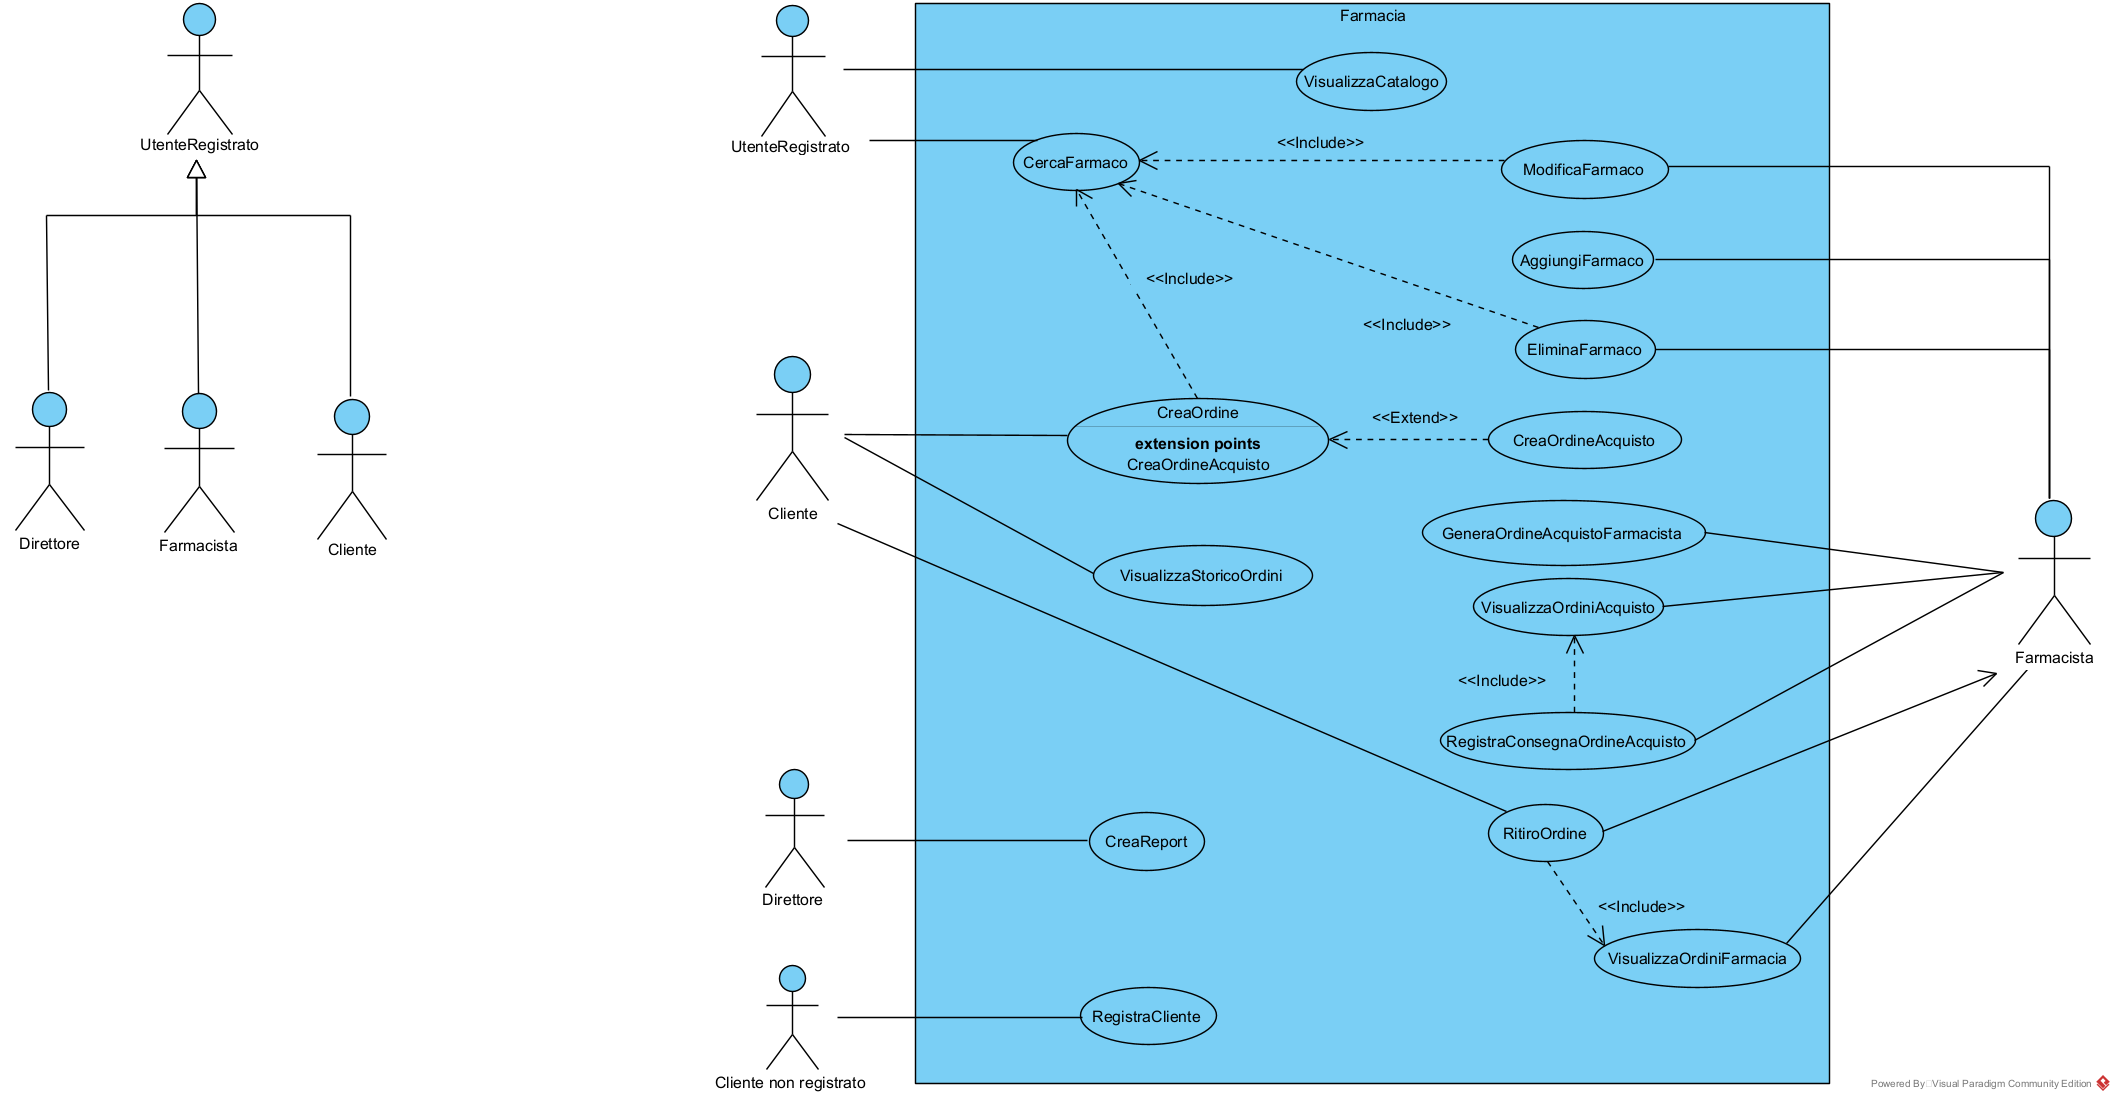
\includegraphics[width=\linewidth]{assets/UseCaseFarmacia.png}

\pagebreak

\section{Scenari}

\IncludeTable[!hbp]{chapters/usecases/RegistraCliente} % input
\IncludeTable[!hbp]{chapters/usecases/AggiungiFarmaco}
\IncludeTable[!hbp]{chapters/usecases/CercaFarmaco}
\IncludeTable[!hbp]{chapters/usecases/ModificaFarmaco}
\IncludeTable[!hbp]{chapters/usecases/EliminaFarmaco}
\IncludeTable[!hpt]{chapters/usecases/VisualizzaCatalogo}
\IncludeTable[!hpt]{chapters/usecases/VisualizzaOrdiniAcquisto}
\IncludeTable[!hpt]{chapters/usecases/RegistraConsegnaOrdineAcquisto}
\IncludeTable[!hpt]{chapters/usecases/VisualizzaOrdiniFarmacia}
\IncludeTable{chapters/usecases/CreaOrdine}
\IncludeTable{chapters/usecases/RitiraOrdine}

\vfill
\pagebreak

\IncludeTable[!ht]{chapters/usecases/VisualizzaStoricoOrdini}
\IncludeTable[!ht]{chapters/usecases/GeneraReport}
\IncludeTable[!ht]{chapters/usecases/GeneraOrdineAcquisto}
\IncludeTable[!ht]{chapters/usecases/GeneraOrdineAcquistoFarmacista}

\vfill
\pagebreak

\section{Diagramma delle Classi}
Di seguito riportiamo il diagramma delle classi di analisi.
\begin{figure}[!ht]
	\centering
	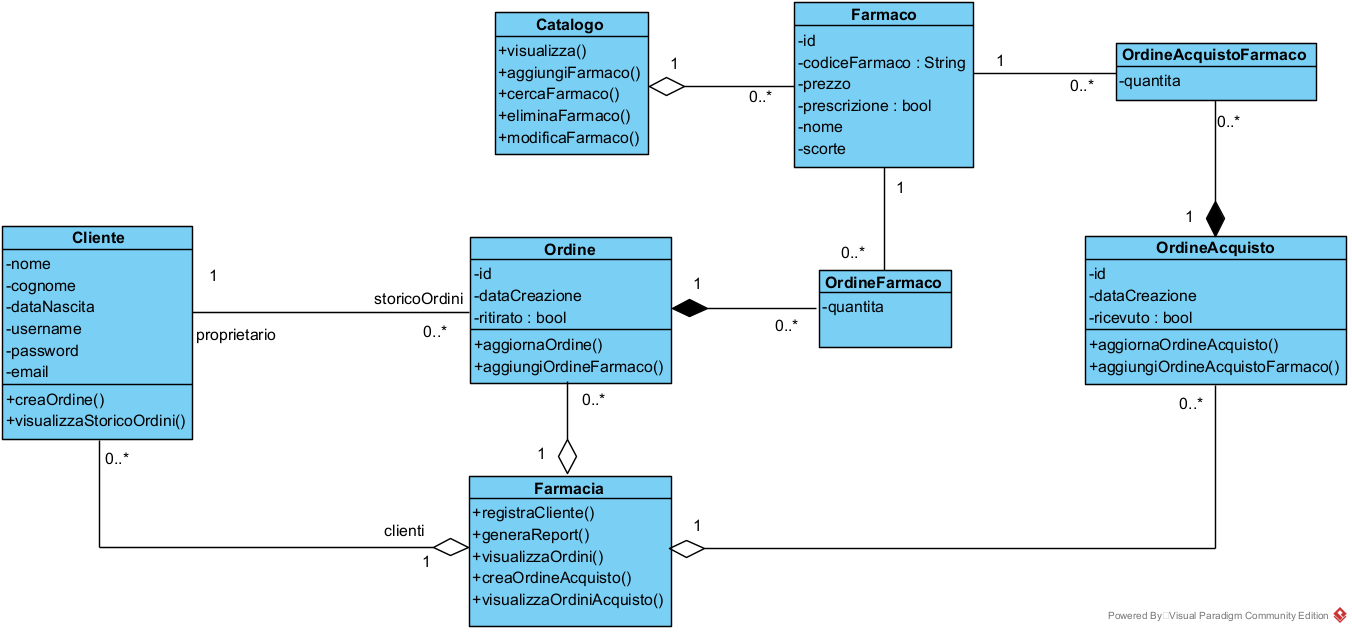
\includegraphics[width=\linewidth]{assets/ClassDiagramAnalisi.png}
	\caption{Diagramma delle classi di analisi}
\end{figure}

\section{Diagrammi di Sequenza}

\begin{figure}[!hbp]
	\centering
	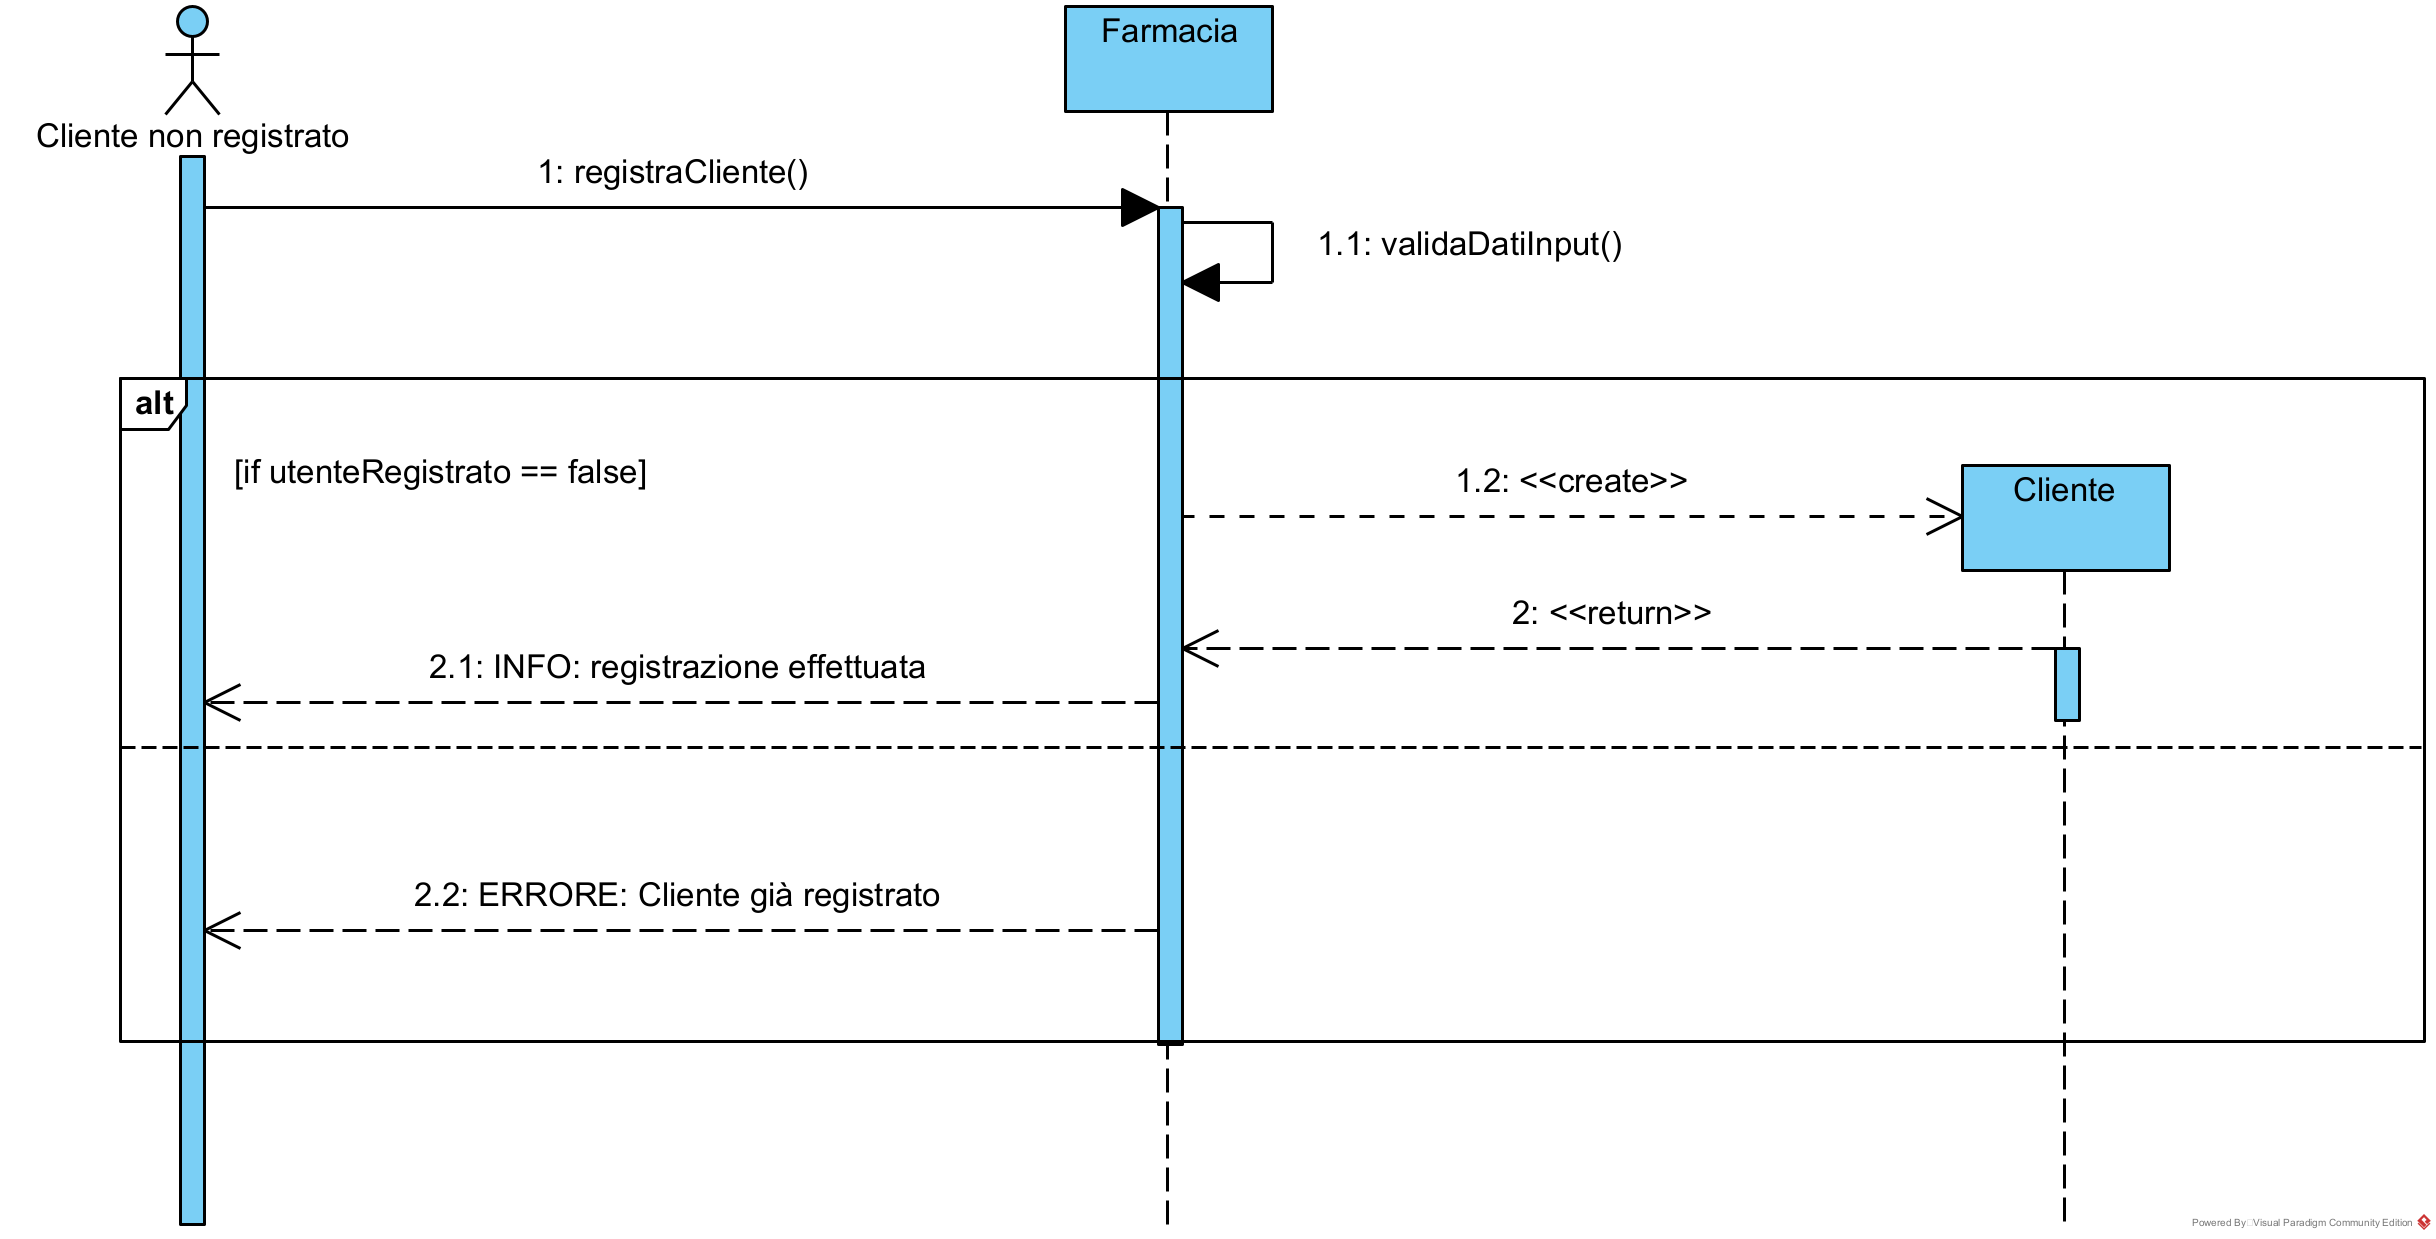
\includegraphics[width=0.8\linewidth]{assets/sequence_analisi/SequenceAnalisiRegistraCliente.png}
	\caption{Diagramma di sequenza di analisi di RegistraCliente}
\end{figure}

\begin{figure}[!hbp]
	\centering
	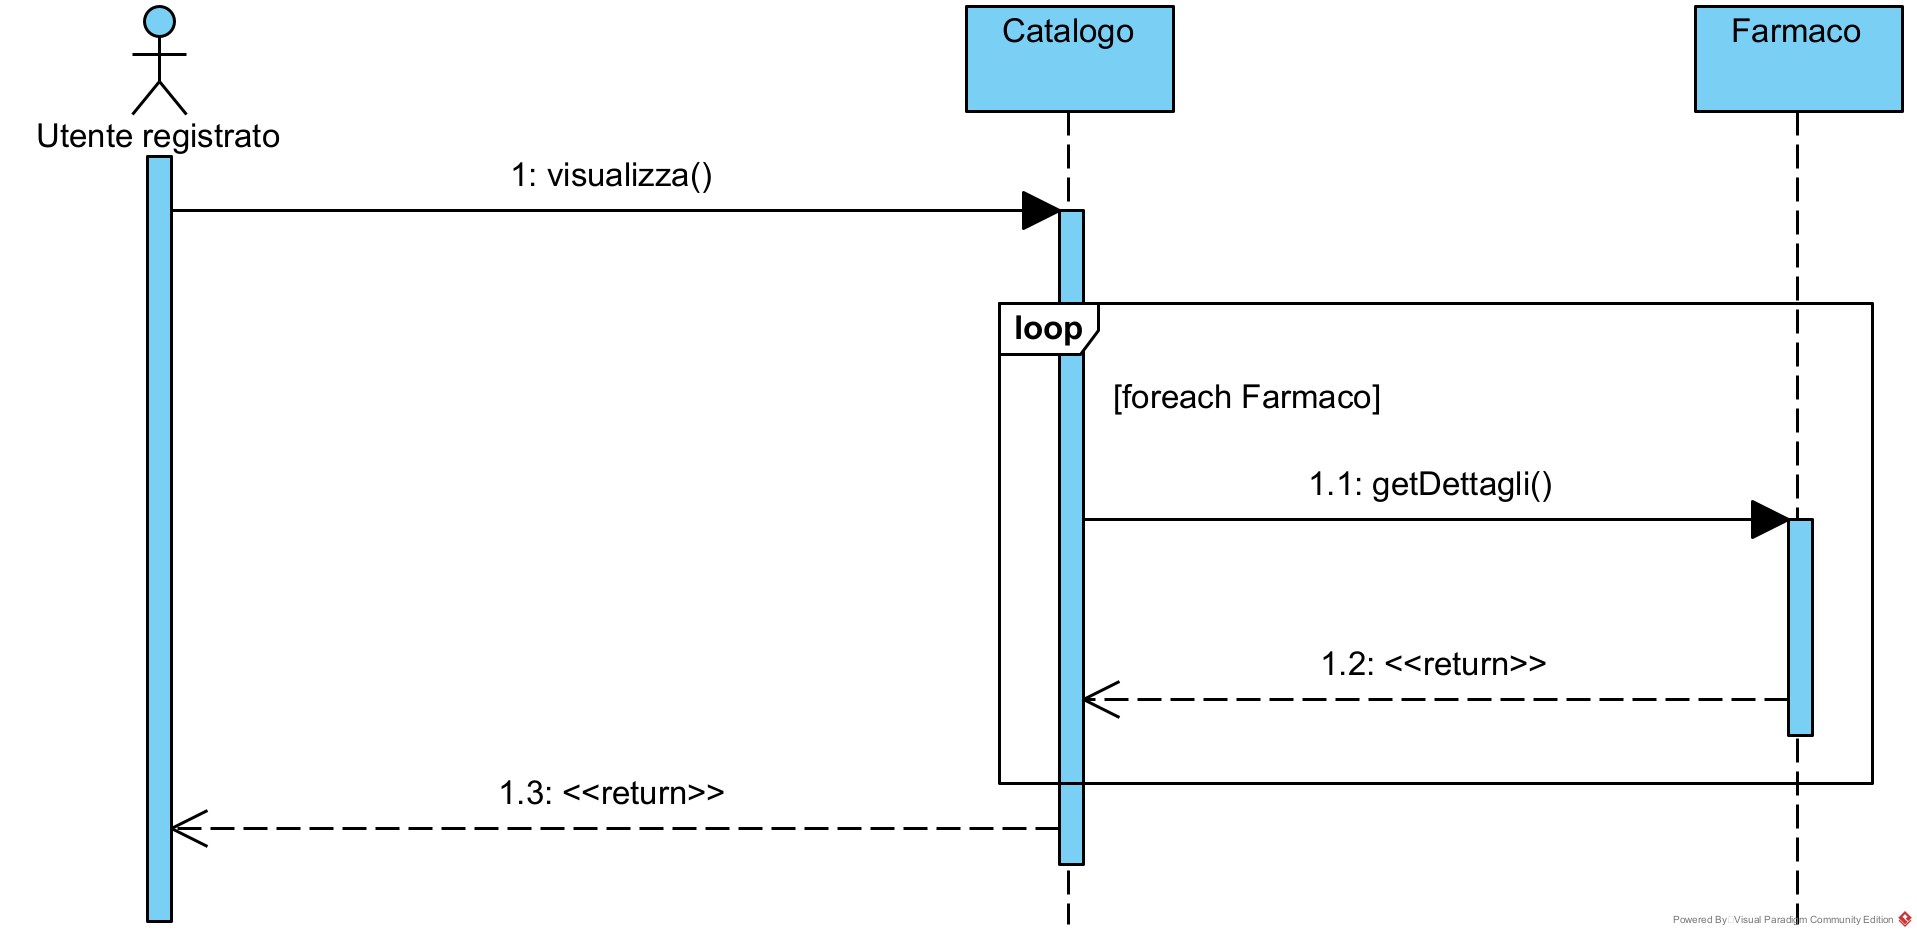
\includegraphics[width=0.8\linewidth]{assets/sequence_analisi/SequenceAnalisiVisualizzaCatalogo.png}
	\caption{Diagramma di sequenza di analisi di VisualizzaCatalogo}
\end{figure}

\begin{figure}[!hbp]
	\centering
	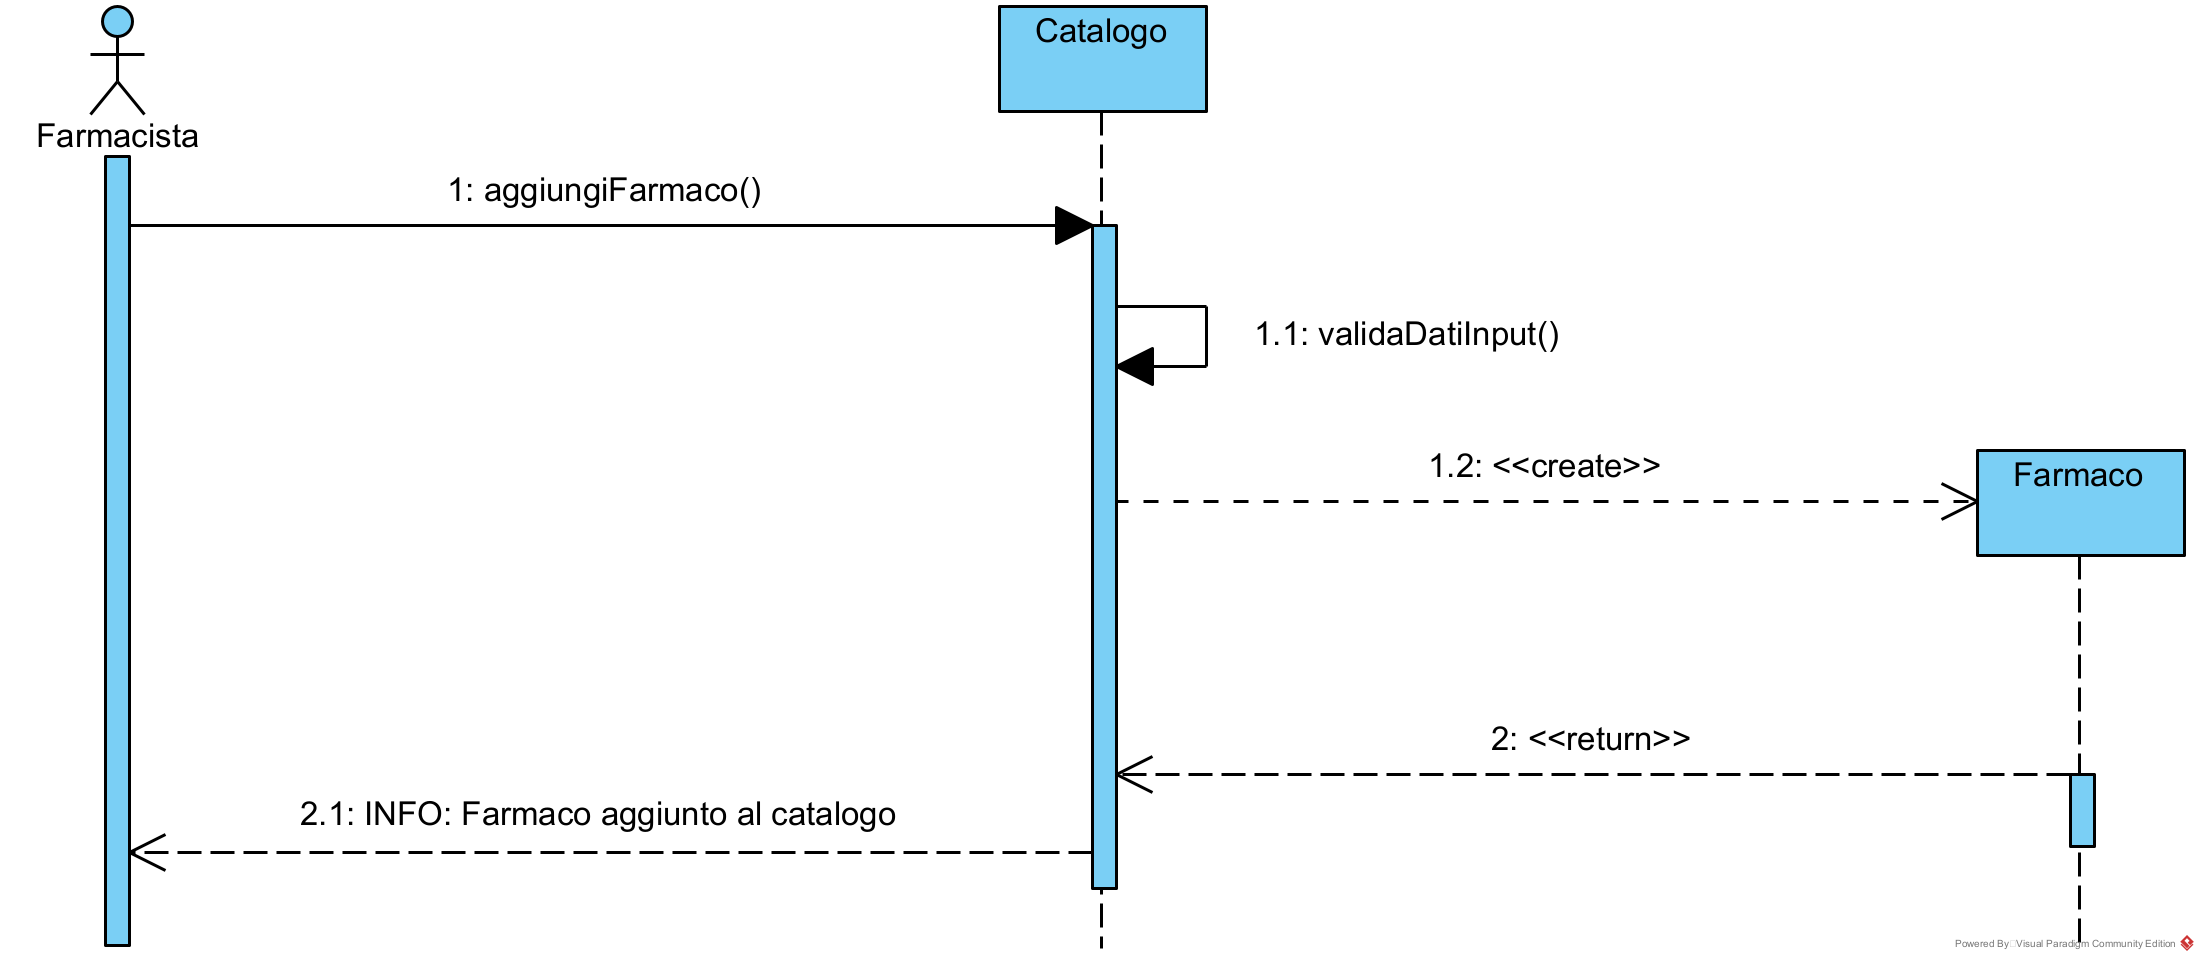
\includegraphics[width=0.8\linewidth]{assets/sequence_analisi/SequenceAnalisiAggiungiFarmaco.png}
	\caption{Diagramma di sequenza di analisi di AggiungiFarmaco}
\end{figure}

\begin{figure}[!hbp]
	\centering
	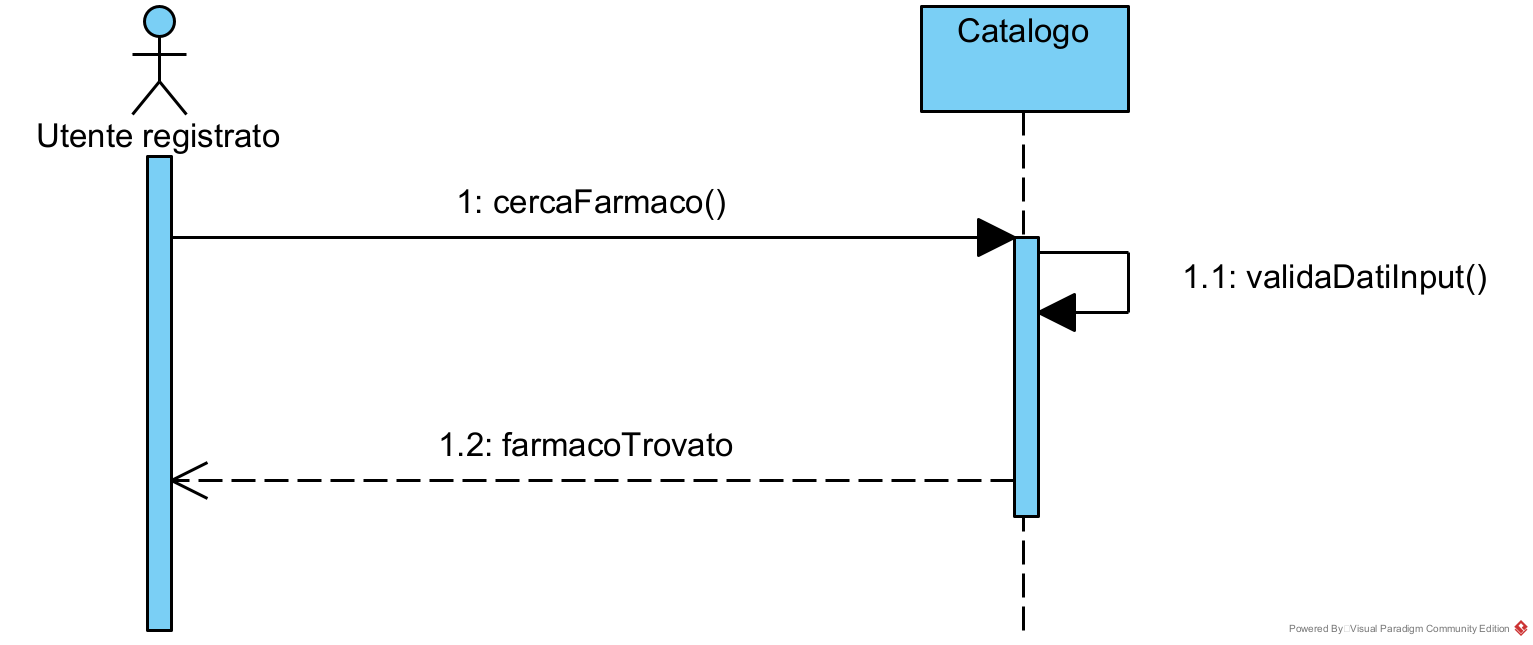
\includegraphics[width=0.7\linewidth]{assets/sequence_analisi/SequenceAnalisiCercaFarmaco.png}
	\caption{Diagramma di sequenza di analisi di CercaFarmaco}
\end{figure}

\begin{figure}[!hbp]
	\centering
	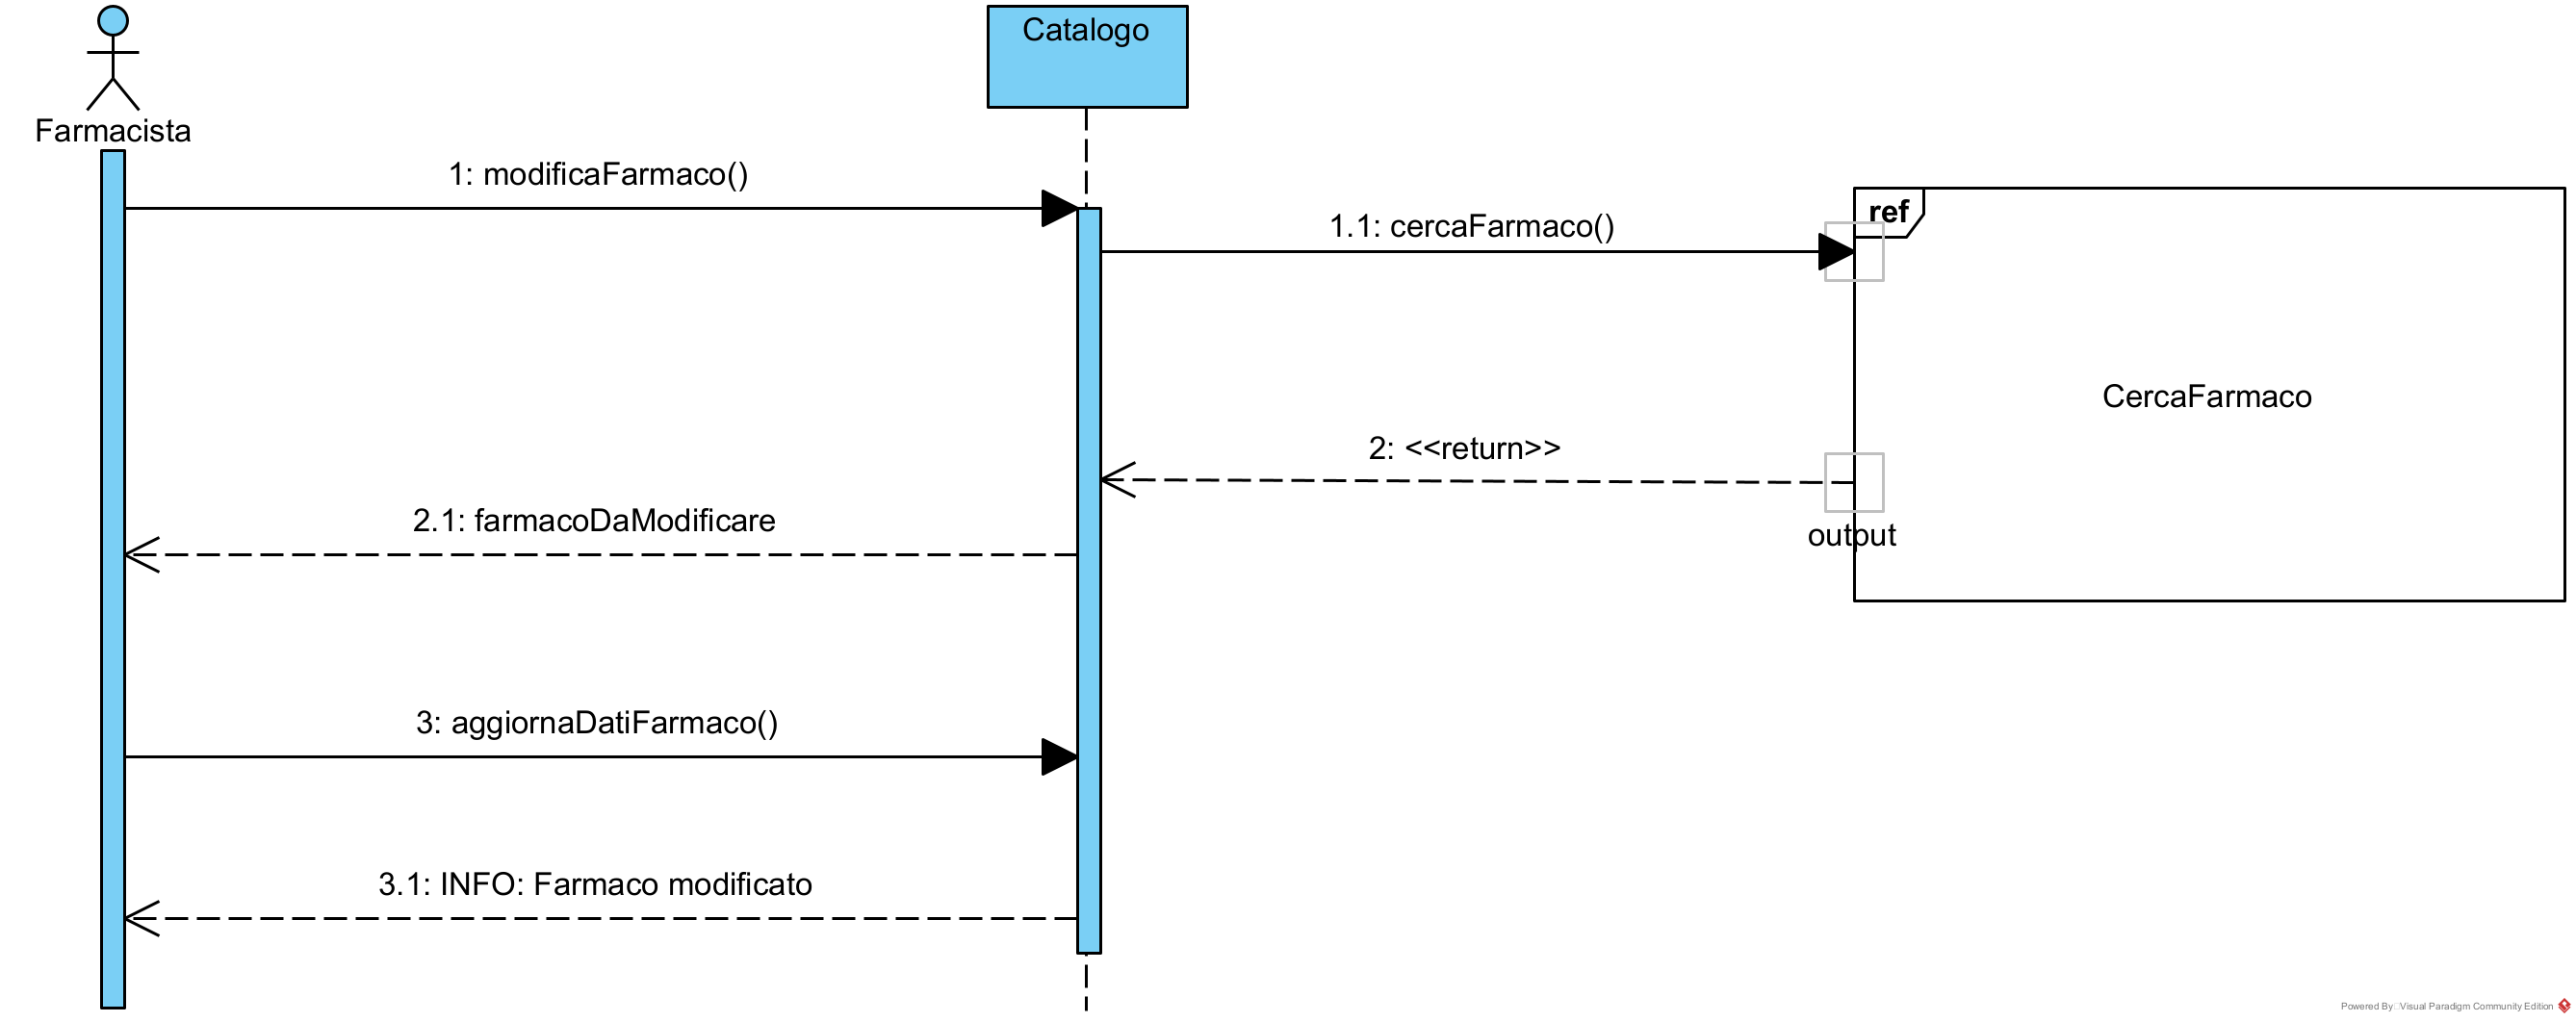
\includegraphics[width=\linewidth]{assets/sequence_analisi/SequenceAnalisiModificaFarmaco.png}
	\caption{Diagramma di sequenza di analisi di ModificaFarmaco}
\end{figure}

\begin{figure}[!hbp]
	\centering
	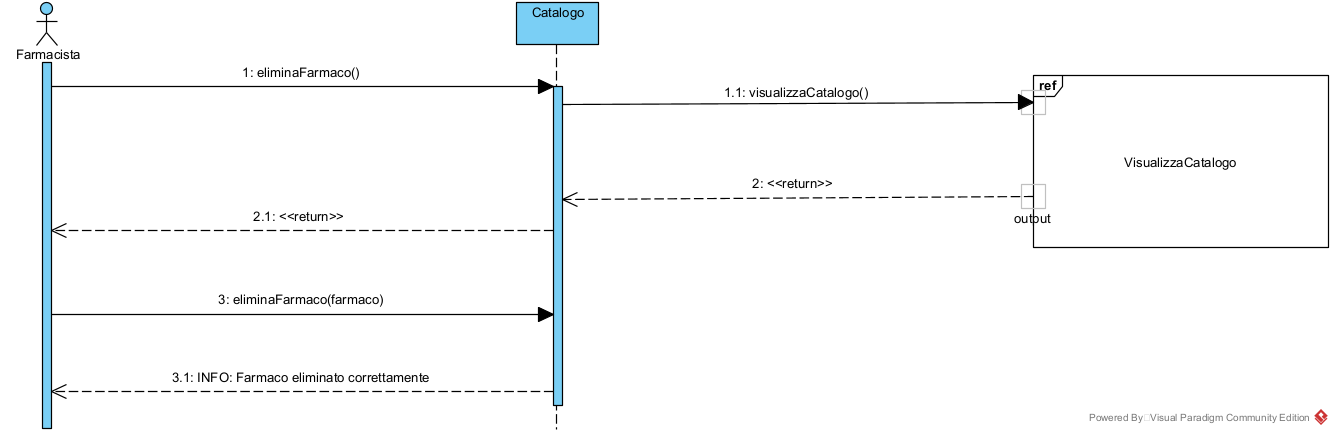
\includegraphics[width=\linewidth]{assets/sequence_analisi/SequenceAnalisiEliminaFarmaco.png}
	\caption{Diagramma di sequenza di analisi di EliminaFarmaco}
\end{figure}

\begin{figure}[!hbp]
	\centering
	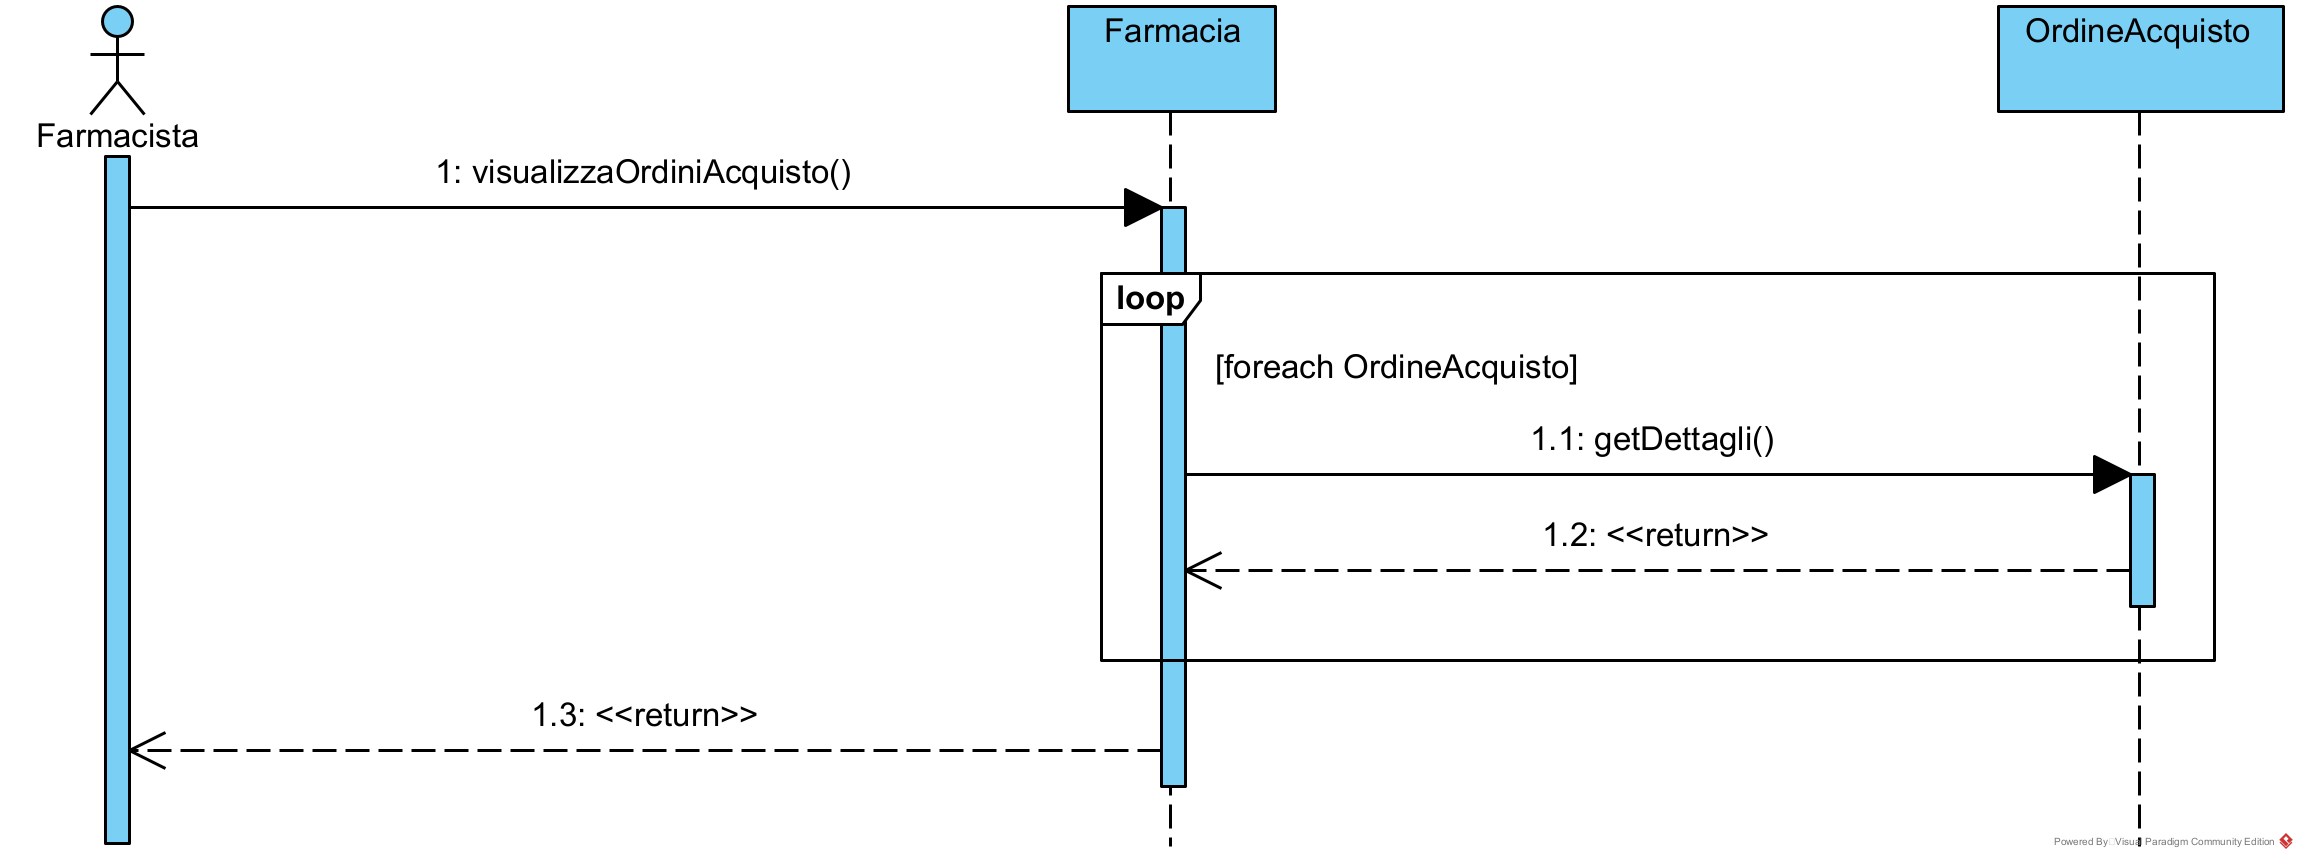
\includegraphics[width=0.9\linewidth]{assets/sequence_analisi/SequenceAnalisiVisualizzaOrdiniAcquisto.png}
	\caption{Diagramma di sequenza di analisi di VisualizzaOrdiniAcquisto}
\end{figure}

\begin{figure}[!hbp]
	\centering
	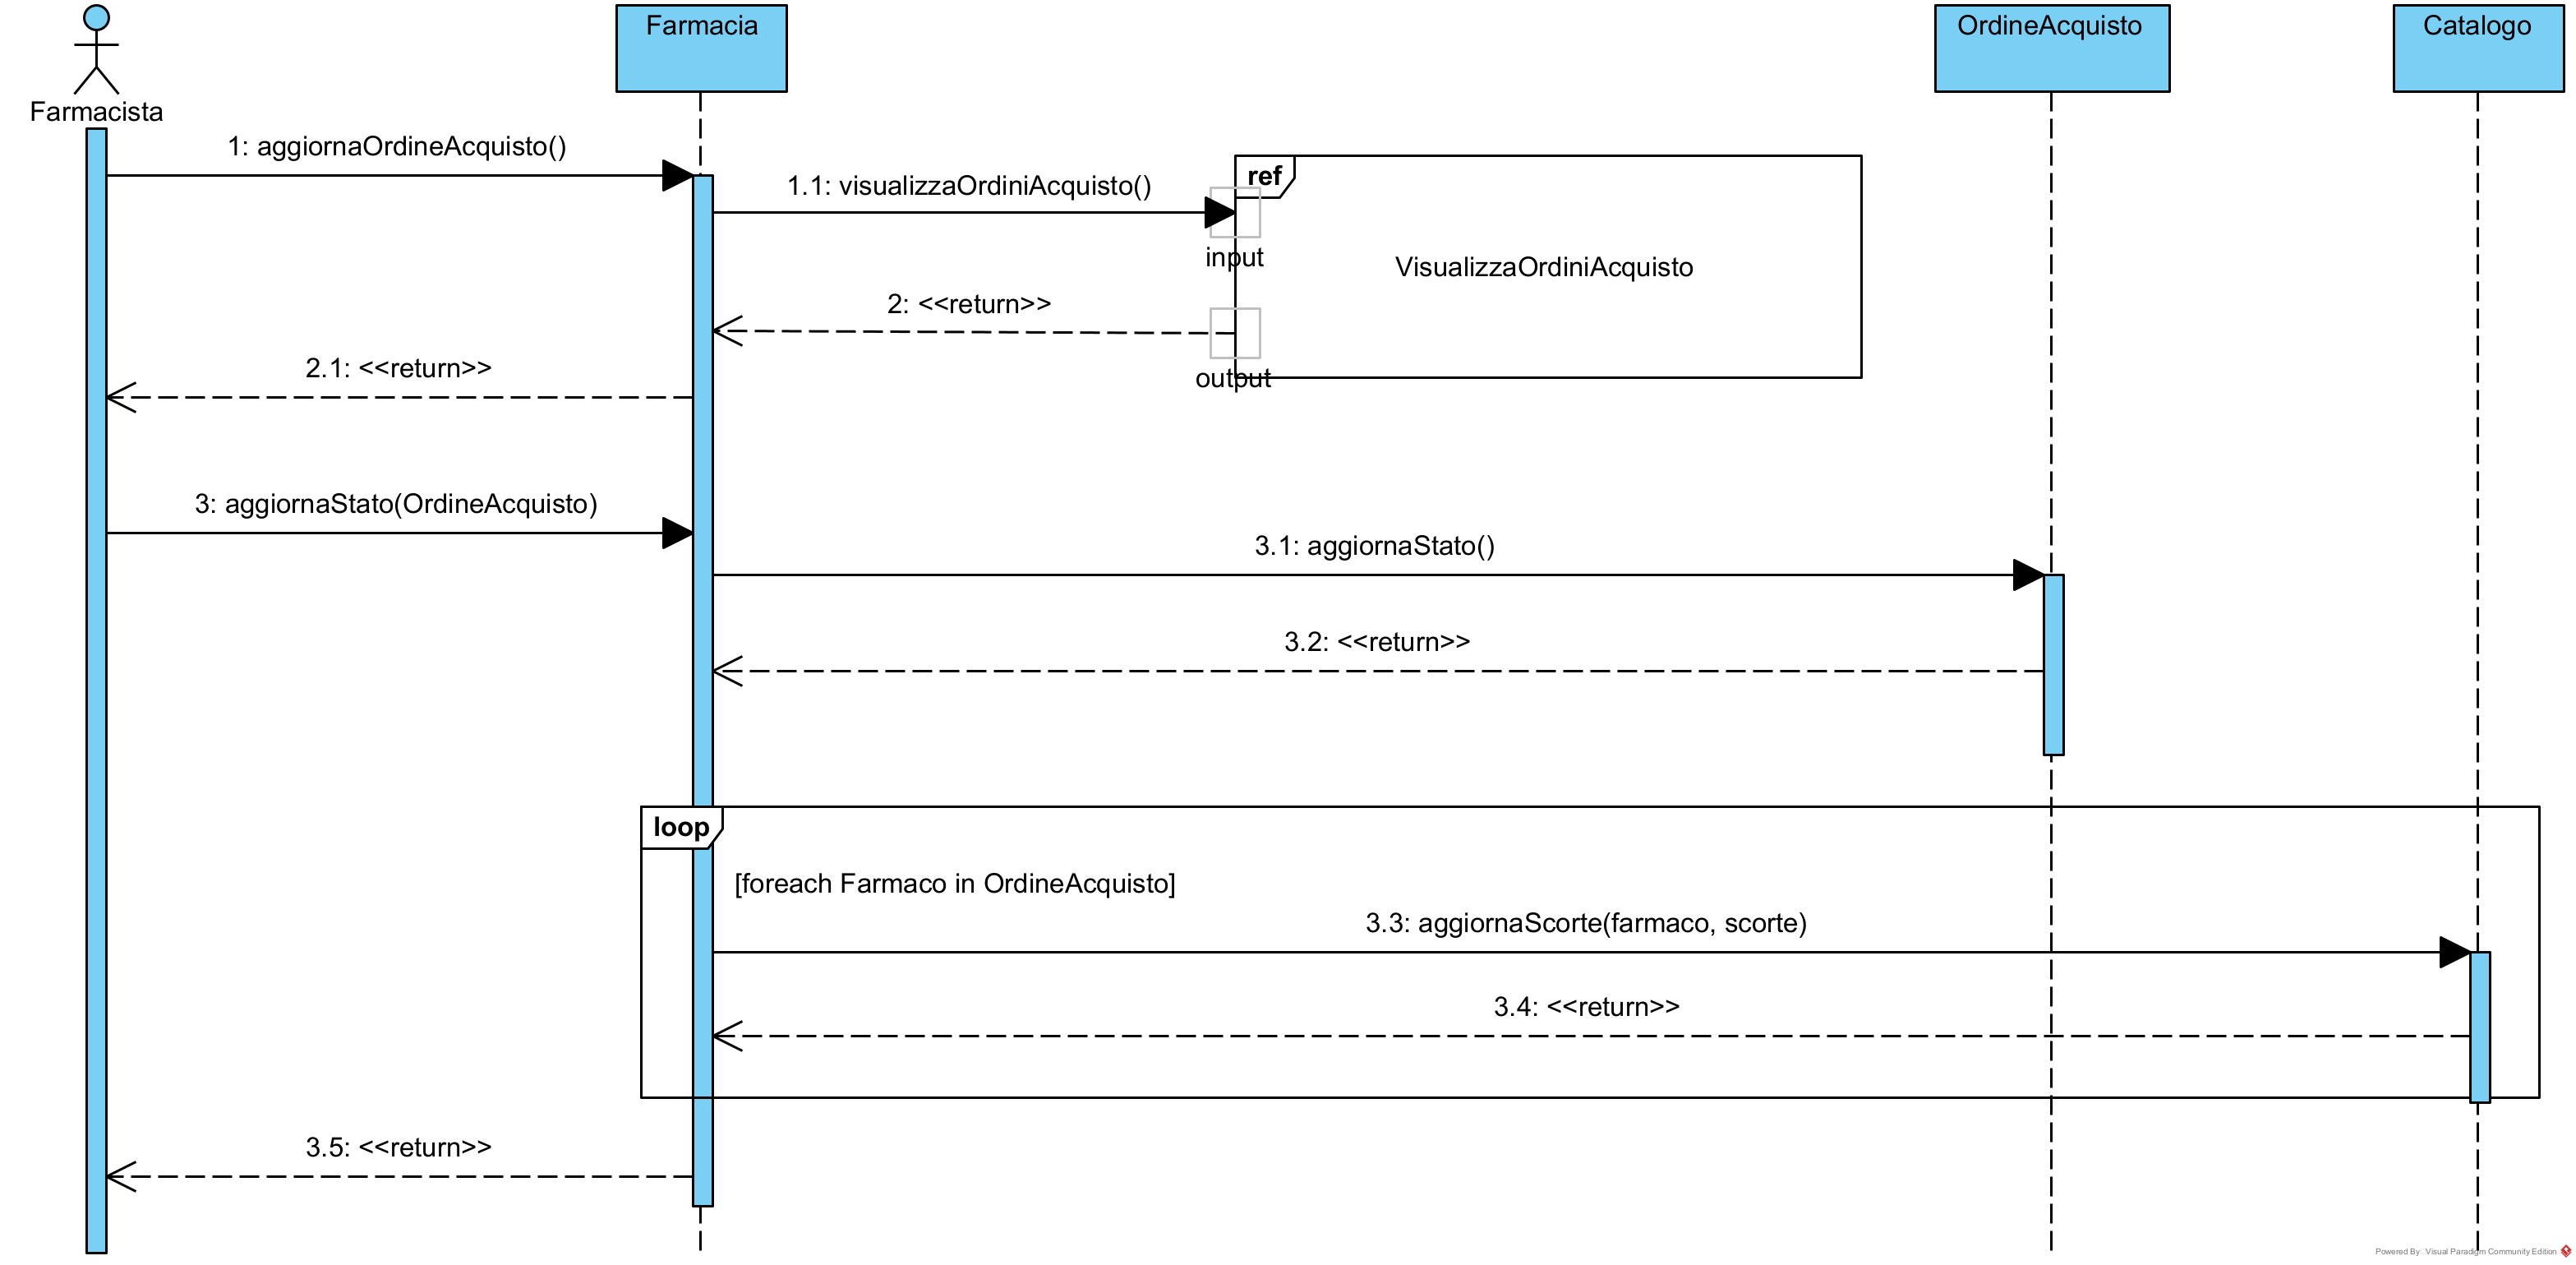
\includegraphics[width=\linewidth]{assets/sequence_analisi/SequenceAnalisiAggiornaOrdineAcquisto.png}
	\caption{Diagramma di sequenza di analisi di AggiornaOrdineAcquisto (RegistraConsegnaOrdineAcquisto)}
\end{figure}

\begin{figure}[!hbp]
	\centering
	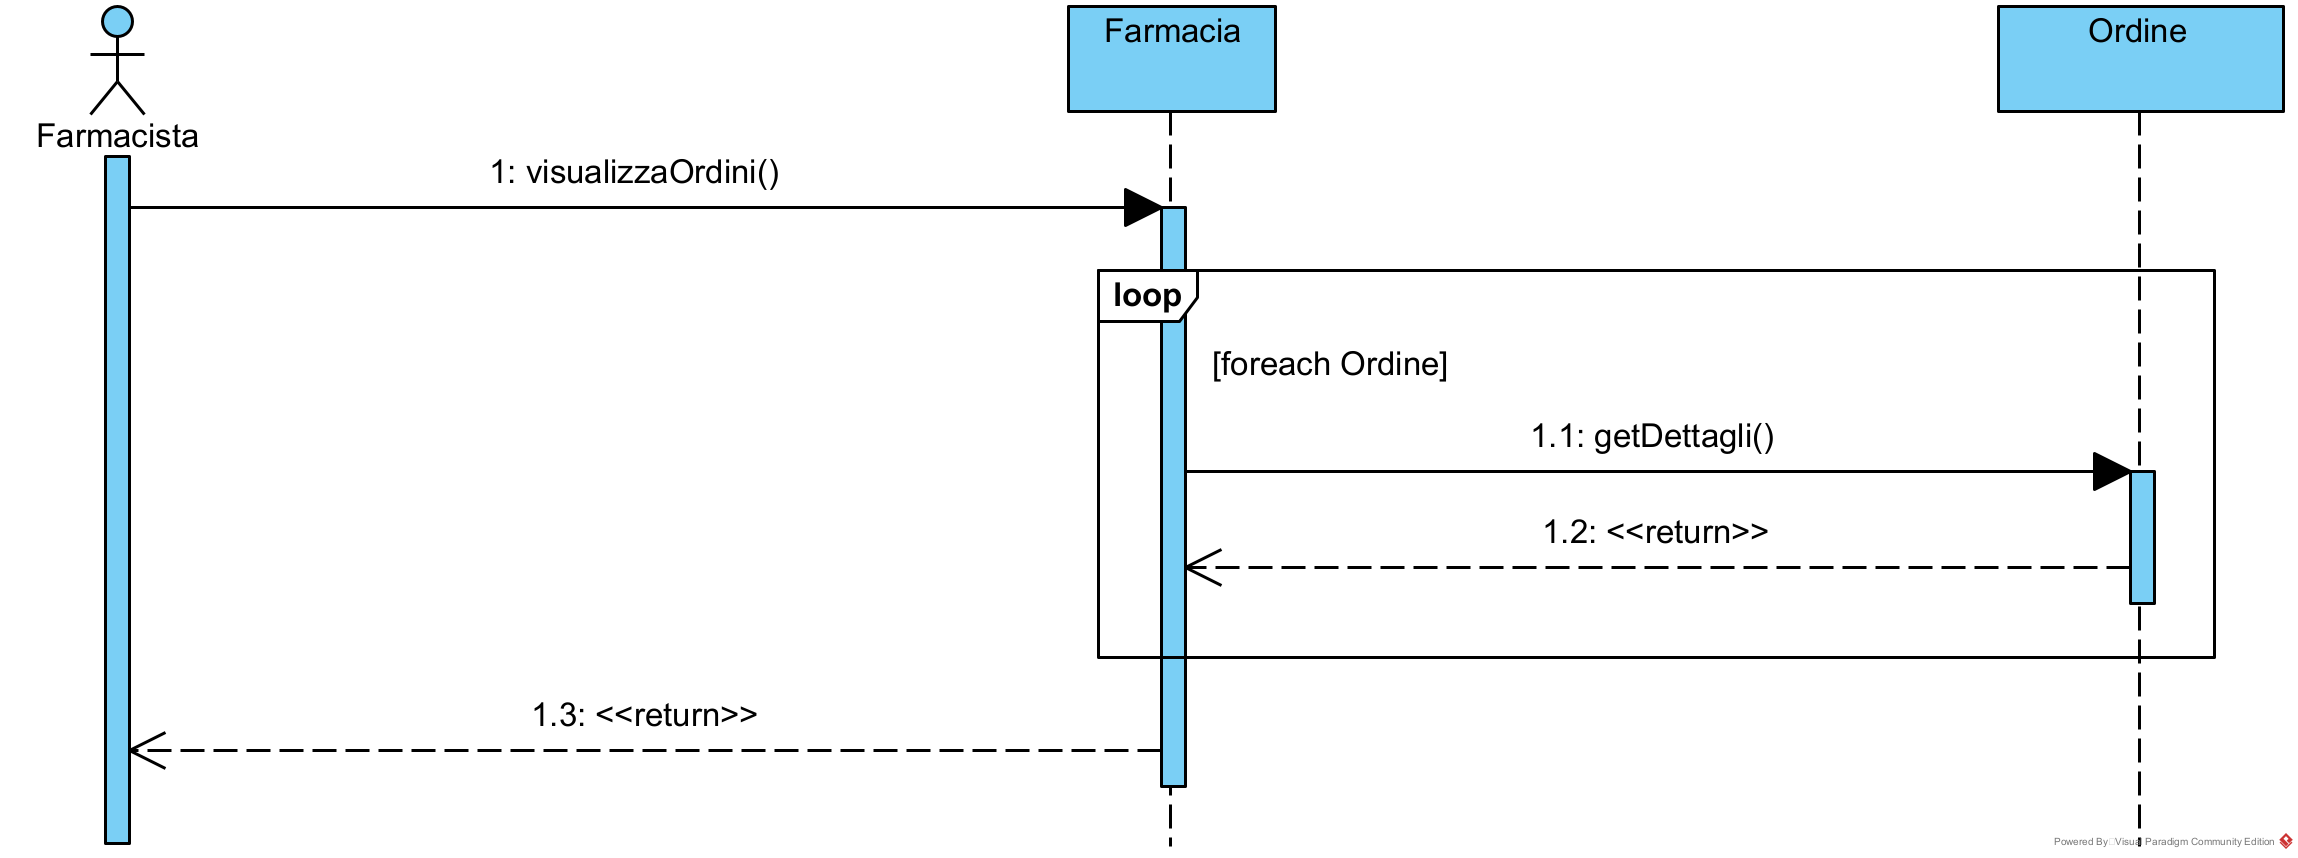
\includegraphics[width=0.9\linewidth]{assets/sequence_analisi/SequenceAnalisiVisualizzaOrdiniFarmacia.png}
	\caption{Diagramma di sequenza di analisi di VisualizzaOrdiniFarmacia}
\end{figure}

\begin{figure}[!hbp]
	\centering
	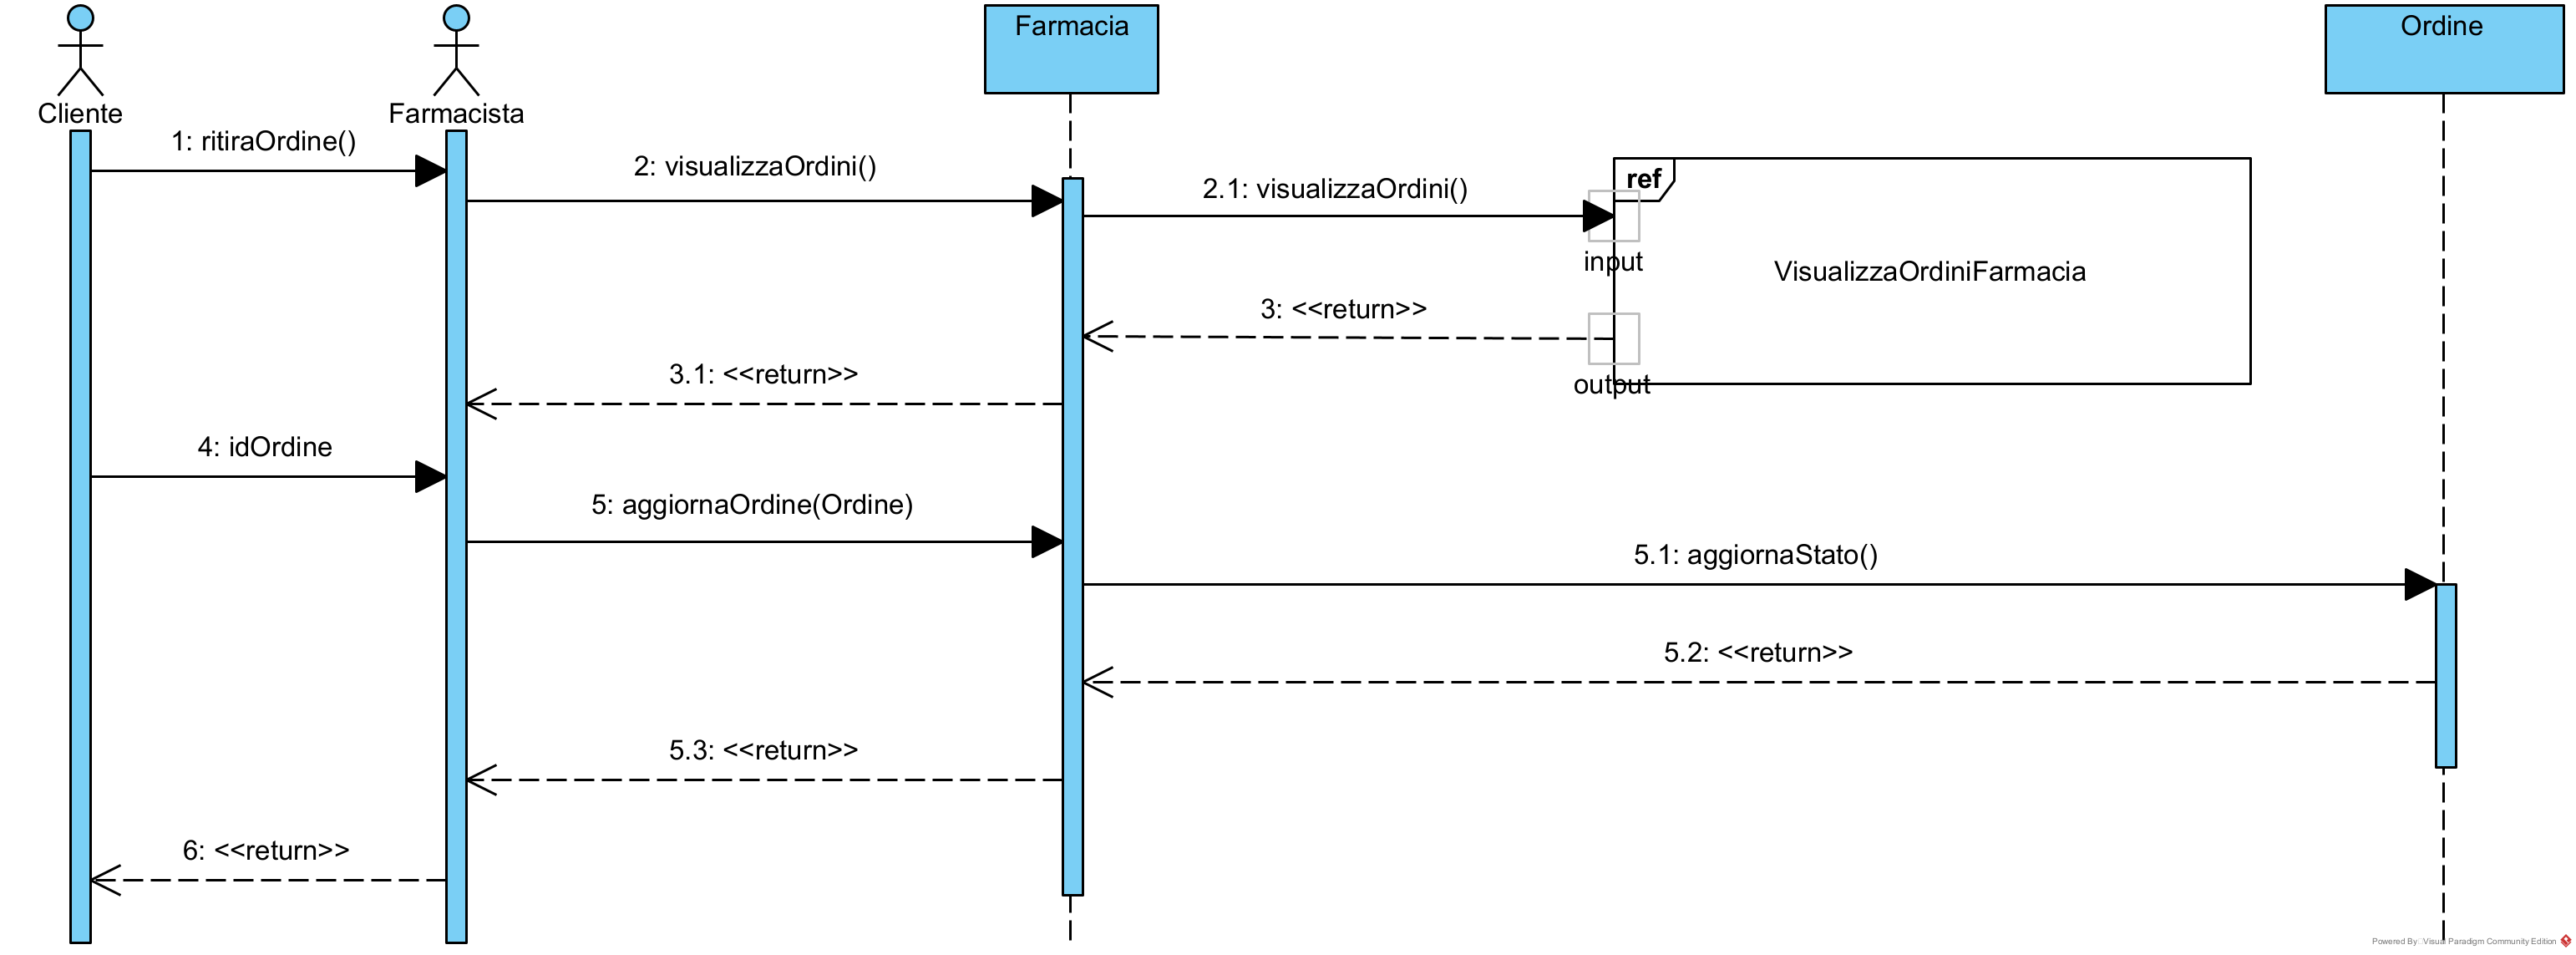
\includegraphics[width=0.8\linewidth]{assets/sequence_analisi/SequenceAnalisiRitiraOrdine.png}
	\caption{Diagramma di sequenza di analisi di RitiraOrdine}
\end{figure}

\begin{figure}[!hbp]
	\centering
	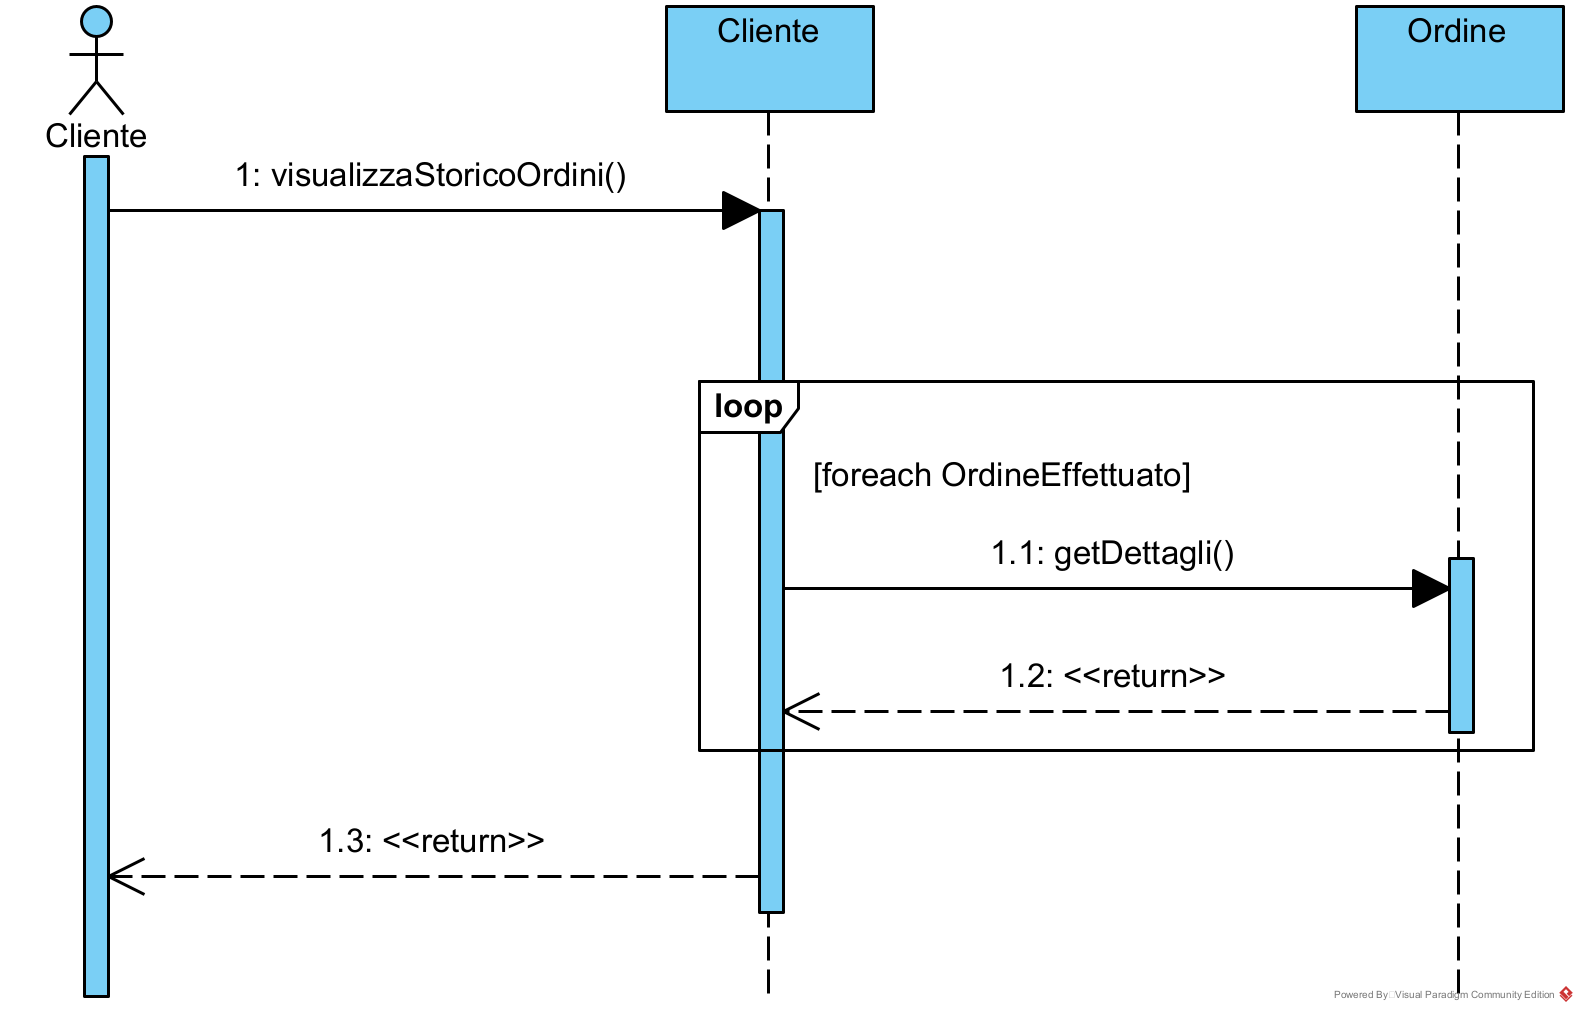
\includegraphics[width=0.8\linewidth]{assets/sequence_analisi/SequenceAnalisiVisualizzaStoricoOrdini.png}
	\caption{Diagramma di sequenza di analisi di VisualizzaStoricoOrdini}
\end{figure}

\begin{figure}[!hbp]
	\centering
	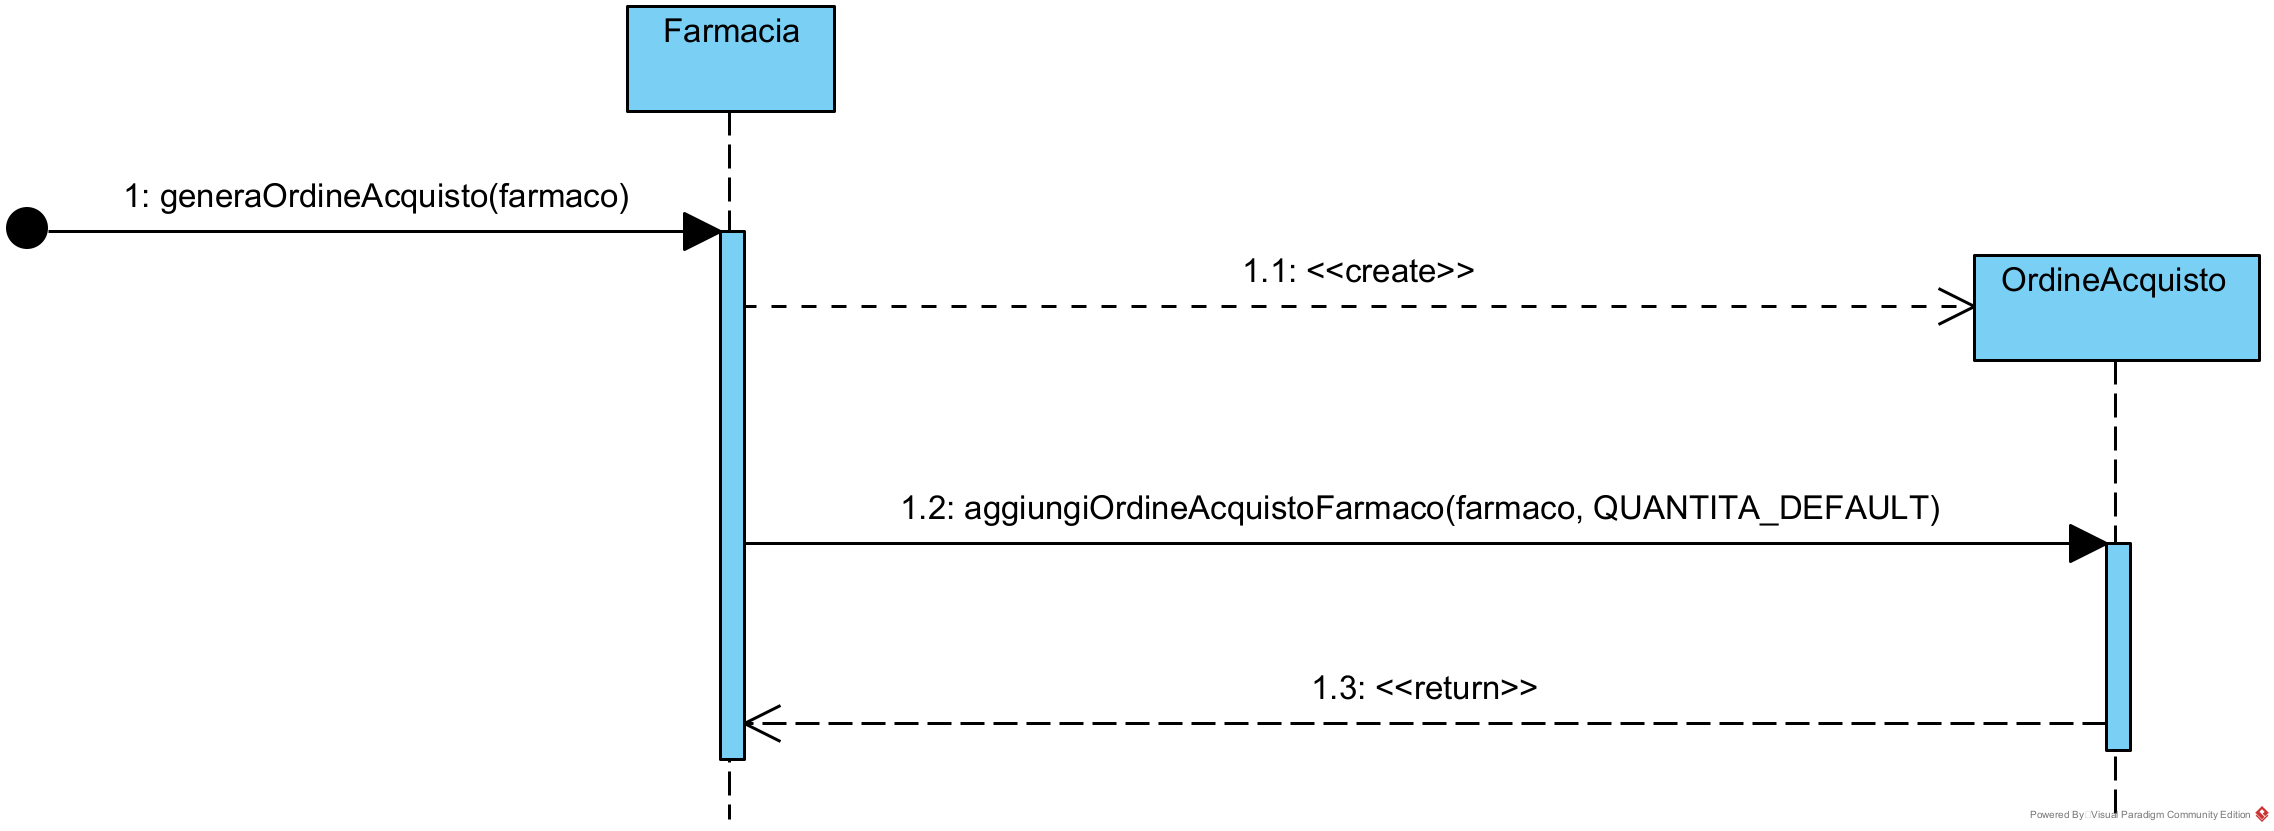
\includegraphics[width=0.8\linewidth]{assets/sequence_analisi/SequenceAnalisiGeneraOrdineAcquisto.png}
	\caption{Diagramma di sequenza di analisi di GeneraOrdineAcquisto}
\end{figure}

\begin{figure}[!hbp]
	\centering
	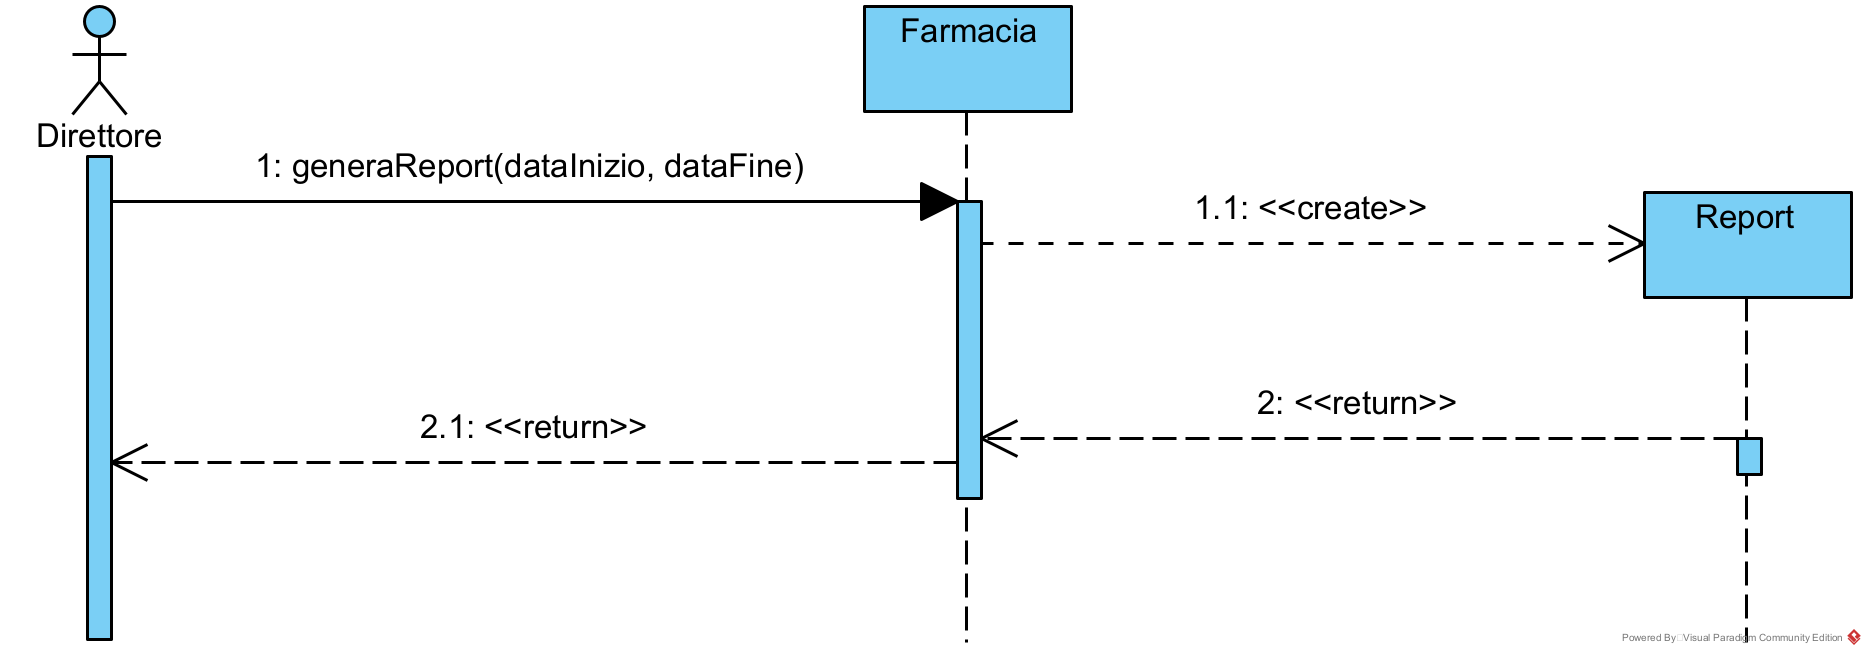
\includegraphics[width=0.8\linewidth]{assets/sequence_analisi/SequenceAnalisiGeneraReport.png}
	\caption{Diagramma di sequenza di analisi di GeneraReport}
\end{figure}

\begin{figure}[!hbp]
	\centering
	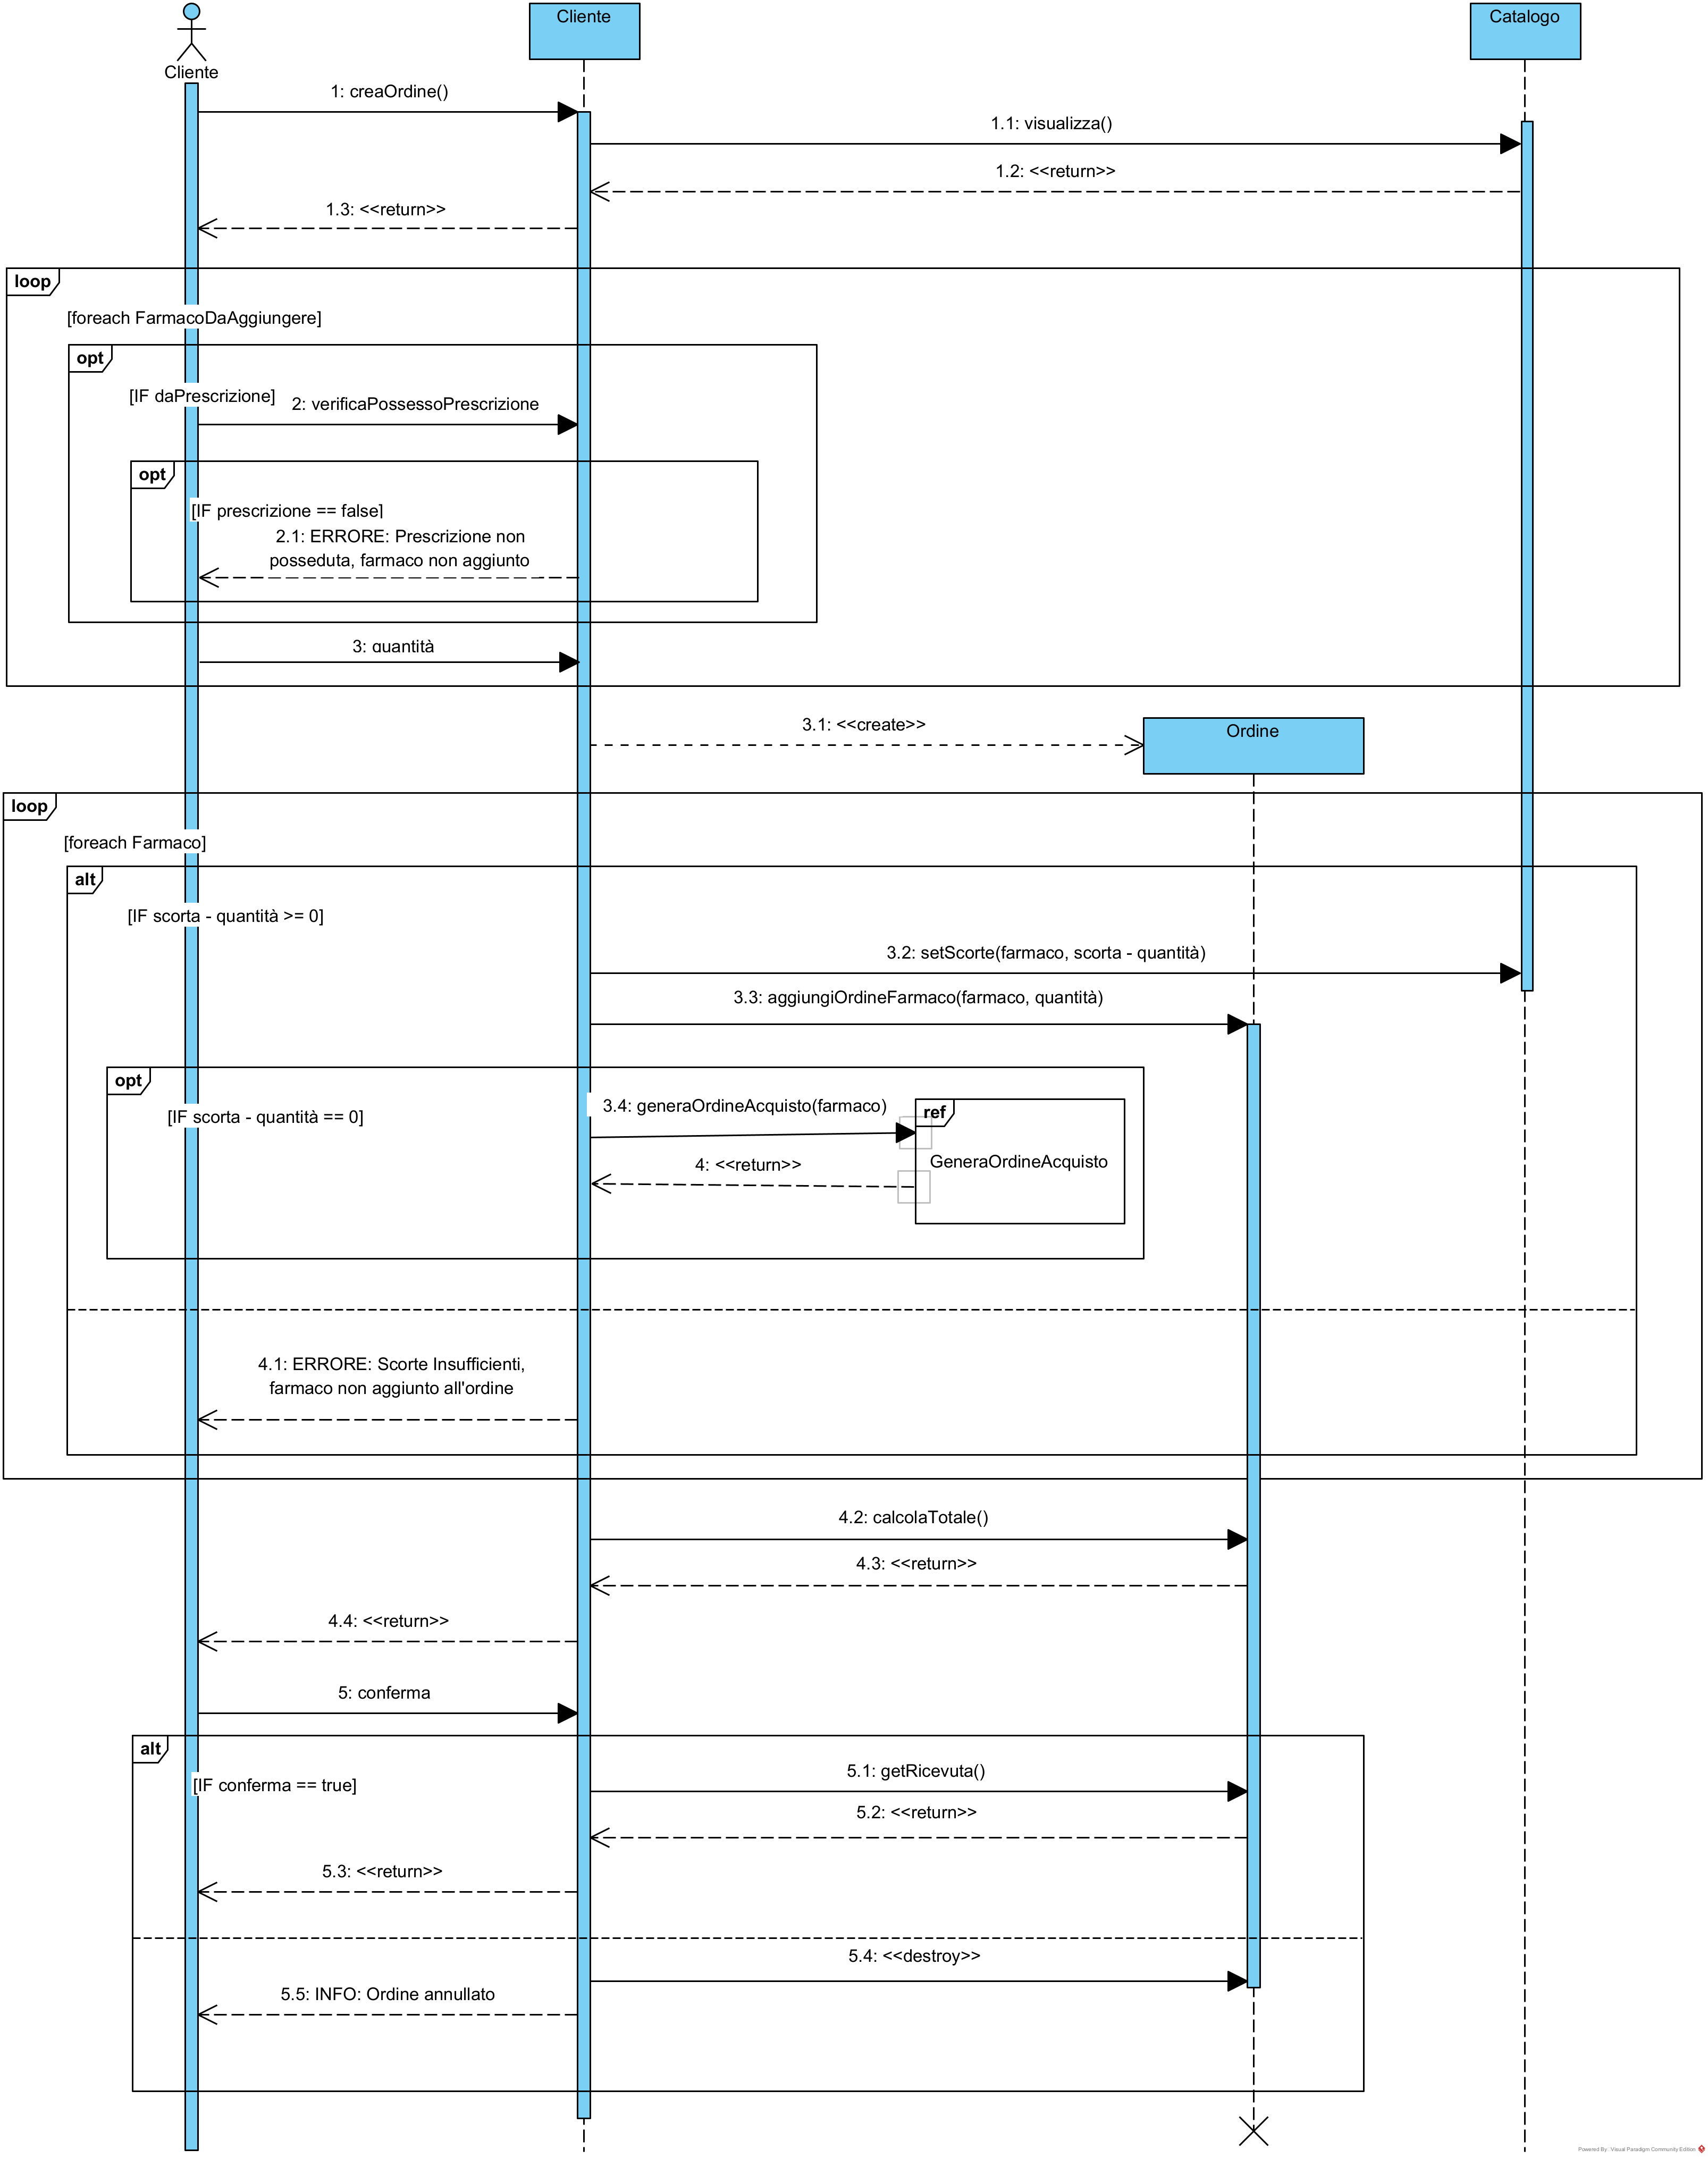
\includegraphics[width=\linewidth]{assets/sequence_analisi/SequenceAnalisiCreaOrdine.png}
	\caption{Diagramma di sequenza di analisi di CreaOrdine}
\end{figure}

\begin{figure}[!ht]
	\centering
	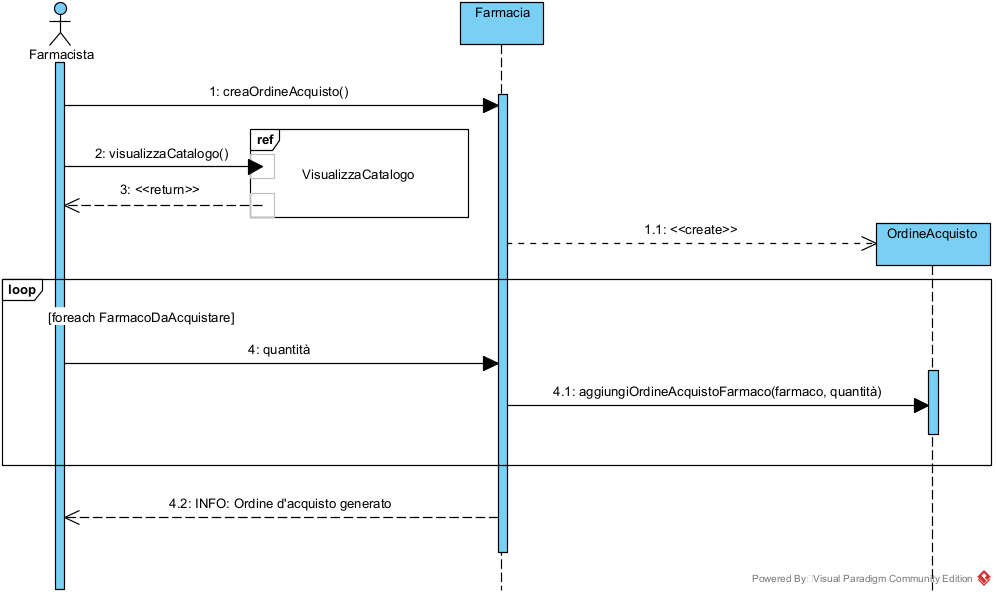
\includegraphics[width=\linewidth]{assets/sequence_analisi/SequenceAnalisiGeneraOrdineAcquistoFarmacista.png}
	\caption{Diagramma di sequenza di analisi di GeneraOrdineAcquistoFarmacista}
\end{figure}

\section{Verifica Completezza dei Requisiti}

\begin{itemize}
	\item \Req{rf}{01}, \Req{rf}{06} Modellati in UCD da VisualizzaCatalogo con l'attore UtenteRegistrato e con il caso d'uso UC1
	\item \Req{rf}{02} Modellato in UCD da AggiungiFarmaco con l'attore primario Farmacista
	\item \Req{rf}{03} Modellato in UCD da ModificaFarmaco con l'attore primario Farmacista
	\item \Req{rf}{04} Modellato in UCD da EliminaFarmaco con l'attore primario Farmacista
	\item \Req{rf}{05} Modellato in UCD da RegistraCliente con l'attore primario Cliente non Registrato
	\item \Req{rf}{07}, \Req{rf}{08}, \Req{rf}{09}, \Req{rf}{10}, \Req{rf}{17} Modellati in UCD da CreaOrdine con l'attore primario Cliente
	\item \Req{rf}{11} Modellato in UCD da VisualizzaOrdiniAcquisto con l'attore primario Farmacista
	\item \Req{rf}{12} Modellato in UCD da RegistraConsegnaOrdineAcquisto con l'attore primario Farmacista
	\item \Req{rf}{13} Modellato in UCD da GeneraReport con l'attore primario Direttore
	\item \Req{rf}{14} Modellato in UCD da VisualizzaOrdiniFarmacia con l'attore primario Farmacista
	\item \Req{rf}{15} Modellato in UCD da RitiraOrdine con l'attore primario Cliente e attore secondario Farmacista
	\item \Req{rf}{16} Modellato in UCD da VisualizzaStoricoOrdini con l'attore primario Cliente
	\item \Req{rf}{18} Modellato in UCD da CercaFarmaco con l'attore primario UtenteRegistrato
	\item \Req{rf}{19} Modellato in UCD da GeneraOrdineAcquistoFarmacista con l'attore primario Farmacista
	\item \Req{rd}{01}, \Req{rd}{02} Modellato nel CD dalla classe Farmaco
	\item \Req{rd}{03} Modellato nel CD dalla classe Cliente
	\item \Req{rd}{04} Modellato nel CD dalla classe Report
\end{itemize}

\begin{table}[!hbp]
	\centering
	\begin{tblr}{
		colspec = lllll,
		hlines = {1pt}, colsep = 12pt
		}
		UCD = Use Case Diagram &
		CD = Class Diagram &
		SD = Sequence Diagram \\
	\end{tblr}
\end{table}
\chapter{Piano di Test Funzionale}

\section{RegistraCliente}

\subsubsection*{Category Partition Testing}
% \tiny
% \scriptsize
% \footnotesize
% \small
% \normalsize
% \large
% \Large
% \LARGE
% \huge
% \Huge

\begin{table}[!hbp]
	\centering
	\footnotesize
	\begin{tblr}{
		colspec = XXXXXX,
		hlines, vlines,
		row{1} = {font=\bfseries},
		measure=vbox, stretch=-1
		}
		Nome & Cognome & Username & Password & Email & DataNascita \\
		\begin{itemize}[leftmargin=*]
			\item Stringa di caratteri di lunghezza $\leq$ 45
			\item Stringa di caratteri di lunghezza $>$ 45 \texttt{[ERROR]}
			\item Stringa di caratteri vuota \texttt{[ERROR]}
		\end{itemize} &
		\begin{itemize}[leftmargin=*]
			\item Stringa di caratteri di lunghezza $\leq$ 45
			\item Stringa di caratteri di lunghezza $>$ 45 \texttt{[ERROR]}
			\item Stringa di caratteri vuota \texttt{[ERROR]}
		\end{itemize} &
		\begin{itemize}[leftmargin=*]
			\item Stringa di caratteri di lunghezza $\leq$ 45
			\item Stringa di caratteri di lunghezza $>$ 45 \texttt{[ERROR]}
			\item Stringa di caratteri vuota \texttt{[ERROR]}
		\end{itemize} &
		\begin{itemize}[leftmargin=*]
			\item Stringa di caratteri di lunghezza compresa tra 8 e 45
			\item Stringa di caratteri di lunghezza $<$ 8 \texttt{[ERROR]}
			\item Stringa di caratteri di lunghezza $>$ 45 \texttt{[ERROR]}
		\end{itemize} &
		\begin{itemize}[leftmargin=*]
			\item Stringa di caratteri di lunghezza $\leq$ 45
			\item Stringa di caratteri di lunghezza $>$ 45 \texttt{[ERROR]}
			\item Stringa di caratteri vuota \texttt{[ERROR]}
		\end{itemize} &
		\begin{itemize}[leftmargin=*]
			\item Data con formato valido (gg-mm-aaaa)
			\item Data con formato non valido \texttt{[ERROR]}
		\end{itemize}
	\end{tblr}
\end{table}

\noindent Il numero di test da effettuarsi senza particolari vincoli è: $3 \cdot 3 \cdot 3 \cdot 3 \cdot 3 \cdot 2 = 486$.

\noindent Introduciamo i vincoli \texttt{[ERROR]}. Il numero di test da eseguire per testare singolarmente i vincoli è 11 (2 per Nome, 2 per Cognome, 2 per Username, 2 per Password, 2 per Email, 1 per DataNascita).

\noindent Il numero di test risultante è 12: $(1 \cdot 1 \cdot 1 \cdot 1 \cdot 1 \cdot 1) + 11 = 12$.

\subsubsection*{Test Suite}

\begin{table}[!hbp]
	\centering
	\footnotesize
	\begin{tblr}{
			colspec = lXXXlXX,
			hlines, vlines,
			row{1} = {font=\bfseries},
			measure=vbox
		}
		{Test \\ Case \\ ID} & Descrizione & Classi di Equivalenza Coperte & Pre-condizioni & Input & {Output \\ Attesi} & {Post-condizioni \\ Attese} \\
		1 &
		Tutti gli input validi &
		Nome, Cognome, Username, Password, Email, DataNascita validi &
		Il cliente non è ancora registrato nel sistema &
		{Nome: Mario \\ Cognome: Rossi \\ Username: mariorossi \\ Password: miapassword \\ Email: mariorossi@gmail.com \\ DataNascita: 22-06-1989} &
		Registrazione effettuata & Il cliente è stato correttamente registrato nel sistema \\
		2 &
		Nome $>$ 45 caratteri &
		Nome $>$ 45 caratteri \texttt{[ERROR]}, Cognome, Username, Password, Email, DataNascita validi &
		- &
		{Nome: \dots \\ Cognome: Rossi \\ Username: mariorossi \\ Password: miapassword \\ Email: mariorossi@gmail.com \\ DataNascita: 22-06-1989} &
		Nome troppo lungo &
		- \\
		3 &
		Nome assente &
		Nome assente \texttt{[ERROR]}, Cognome, Username, Password, Email, DataNascita validi &
		- &
		{Nome: \\ Cognome: Rossi \\ Username: mariorossi \\ Password: miapassword \\ Email: mariorossi@gmail.com \\ DataNascita: 22-06-1989} &
		Inserire un nome &
		- \\
	\end{tblr}
\end{table}

\begin{table}[!hbp]
	\centering
	\footnotesize
	\begin{tblr}{
			colspec = lXXXlXX,
			hlines, vlines,
			row{1} = {font=\bfseries},
			measure=vbox
		}
		{Test \\ Case \\ ID} & Descrizione & Classi di Equivalenza Coperte & Pre-condizioni & Input & {Output \\ Attesi} & {Post-condizioni \\ Attese} \\
		4 &
		Cognome $>$ 45 caratteri &
		Cognome $>$ 45 caratteri \texttt{[ERROR]}, Nome, Username, Password, Email, DataNascita validi &
		- &
		{Nome: Mario \\ Cognome: \dots \\ Username: mariorossi \\ Password: miapassword \\ Email: mariorossi@gmail.com \\ DataNascita: 22-06-1989} &
		Cognome troppo lungo &
		- \\
		5 &
		Cognome assente &
		Cognome assente \texttt{[ERROR]}, Nome, Username, Password, Email, DataNascita validi &
		- &
		{Nome: Mario \\ Cognome: \\ Username: mariorossi \\ Password: miapassword \\ Email: mariorossi@gmail.com \\ DataNascita: 22-06-1989} &
		Inserire un cognome &
		- \\
		6 &
		Username $>$ 45 caratteri &
		Username $>$ 45 caratteri \texttt{[ERROR]}, Nome, Cognome, Password, Email, DataNascita validi &
		- &
		{Nome: Mario \\ Cognome: Rossi \\ Username: \dots \\ Password: miapassword \\ Email: mariorossi@gmail.com \\ DataNascita: 22-06-1989} &
		Username troppo lungo &
		- \\
		7 &
		Username assente &
		Username assente \texttt{[ERROR]}, Nome, Cognome, Password, Email, DataNascita validi &
		- &
		{Nome: Mario \\ Cognome: Rossi \\ Username: \\ Password: miapassword \\ Email: mariorossi@gmail.com \\ DataNascita: 22-06-1989} &
		Inserire un username &
		- \\
		8 &
		Password $<$ 8 caratteri &
		Password $<$ 8 caratteri \texttt{[ERROR]}, Nome, Cognome, Username, Email, DataNascita validi &
		- &
		{Nome: Mario \\ Cognome: Rossi \\ Username: mariorossi \\ Password: prova \\ Email: mariorossi@gmail.com \\ DataNascita: 22-06-1989} &
		Password troppo corta &
		- \\
		9 &
		Password $>$ 45 caratteri &
		Password $>$ 45 caratteri \texttt{[ERROR]}, Nome, Cognome, Username, Email, DataNascita validi &
		- &
		{Nome: Mario \\ Cognome: Rossi \\ Username: mariorossi \\ Password: \dots \\ Email: mariorossi@gmail.com \\ DataNascita: 22-06-1989} &
		Password troppo lunga &
		- \\
		10 &
		Email $>$ 45 caratteri &
		Email $>$ 45 caratteri \texttt{[ERROR]}, Nome, Cognome, Username, Password, DataNascita validi &
		- &
		{Nome: Mario \\ Cognome: Rossi \\ Username: mariorossi \\ Password: miapassword \\ Email: \dots \\ DataNascita: 22-06-1989} &
		Email troppo lunga &
		- \\
		11 &
		Email assente &
		Email assente \texttt{[ERROR]}, Nome, Cognome, Username, Password, DataNascita validi &
		- &
		{Nome: Mario \\ Cognome: Rossi \\ Username: \\ Password: miapassword \\ Email: \\ DataNascita: 22-06-1989} &
		Inserire un'email &
		- \\
		12 &
		Formato DataNascita non valida &
		Formato DataNascita non valida \texttt{[ERROR]}, Nome, Cognome, Username, Password, Email validi &
		- &
		{Nome: Mario \\ Cognome: Rossi \\ Username: mariorossi \\ Password: miapassword \\ Email: mariorossi@gmail.com \\ DataNascita: 1989-06-22} &
		Formato data non valido &
		- \\
	\end{tblr}
\end{table}

\section{LoginUtente}

\subsubsection*{Category Partition Testing}
% \tiny
% \scriptsize
% \footnotesize
% \small
% \normalsize
% \large
% \Large
% \LARGE
% \huge
% \Huge

\begin{table}[!hbp]
	\centering
	\footnotesize
	\begin{tblr}{
		colspec = XX,
		hlines, vlines,
		row{1} = {font=\bfseries},
		measure=vbox, stretch=-1
		}
		Username & Password \\
		\begin{itemize}[leftmargin=*]
			\item Stringa di caratteri di lunghezza $\leq$ 45
			\item Stringa di caratteri di lunghezza $>$ 45 \texttt{[ERROR]}
			\item Stringa di caratteri vuota \texttt{[ERROR]}
		\end{itemize} &
		\begin{itemize}[leftmargin=*]
			\item Stringa di caratteri di lunghezza compresa tra 8 e 45
			\item Stringa di caratteri di lunghezza $<$ 8 \texttt{[ERROR]}
			\item Stringa di caratteri di lunghezza $>$ 45 \texttt{[ERROR]}
		\end{itemize}
	\end{tblr}
\end{table}

\noindent Il numero di test da effettuarsi senza particolari vincoli è: $3 \cdot 3 = 9$.

\noindent Introduciamo i vincoli \texttt{[ERROR]}. Il numero di test da eseguire per testare singolarmente i vincoli è 4 (2 per Username, 2 per Password).

\noindent Il numero di test risultante è 5: $(1 \cdot 1) + 4 = 5$.

\subsubsection*{Test Suite}

\begin{table}[!hbp]
	\centering
	\footnotesize
	\begin{tblr}{
			colspec = lXXllXX,
			hlines, vlines,
			row{1} = {font=\bfseries},
			measure=vbox
		}
		{Test \\ Case \\ ID} & Descrizione & Classi di Equivalenza Coperte & Pre-condizioni & Input & {Output \\ Attesi} & {Post-condizioni \\ Attese} \\
		1 &
		Tutti gli input validi &
		Username, Password validi &
		{L'utente deve essere \\ correttamente \\ registrato nel sistema} &
		{Username: mariorossi \\ Password: miapassword} &
		Login effettuato & L'utente è entrato correttamente nel sistema \\
		2 &
		Username $>$ 45 caratteri &
		Username $>$ 45 caratteri \texttt{[ERROR]}, Password valida &
		- &
		{Username: \dots \\ Password: miapassword} &
		Username troppo lungo &
		- \\
		3 &
		Username assente &
		Username assente \texttt{[ERROR]}, Password valida &
		- &
		{Username: \\ Password: miapassword} &
		Inserire un username &
		- \\
		4 &
		Password $<$ 8 caratteri &
		Password $<$ 8 caratteri \texttt{[ERROR]}, Username valido &
		- &
		{Username: mariorossi \\ Password: prova} &
		Password troppo corta &
		- \\
		5 &
		Password $>$ 45 caratteri &
		Password $>$ 45 caratteri \texttt{[ERROR]}, Username valido &
		- &
		{Username: mariorossi \\ Password: \dots} &
		Password troppo lunga &
		- \\
	\end{tblr}
\end{table}
\chapter{Progettazione}

\section{Diagramma delle classi}

\begin{figure}[h]
    \centering
	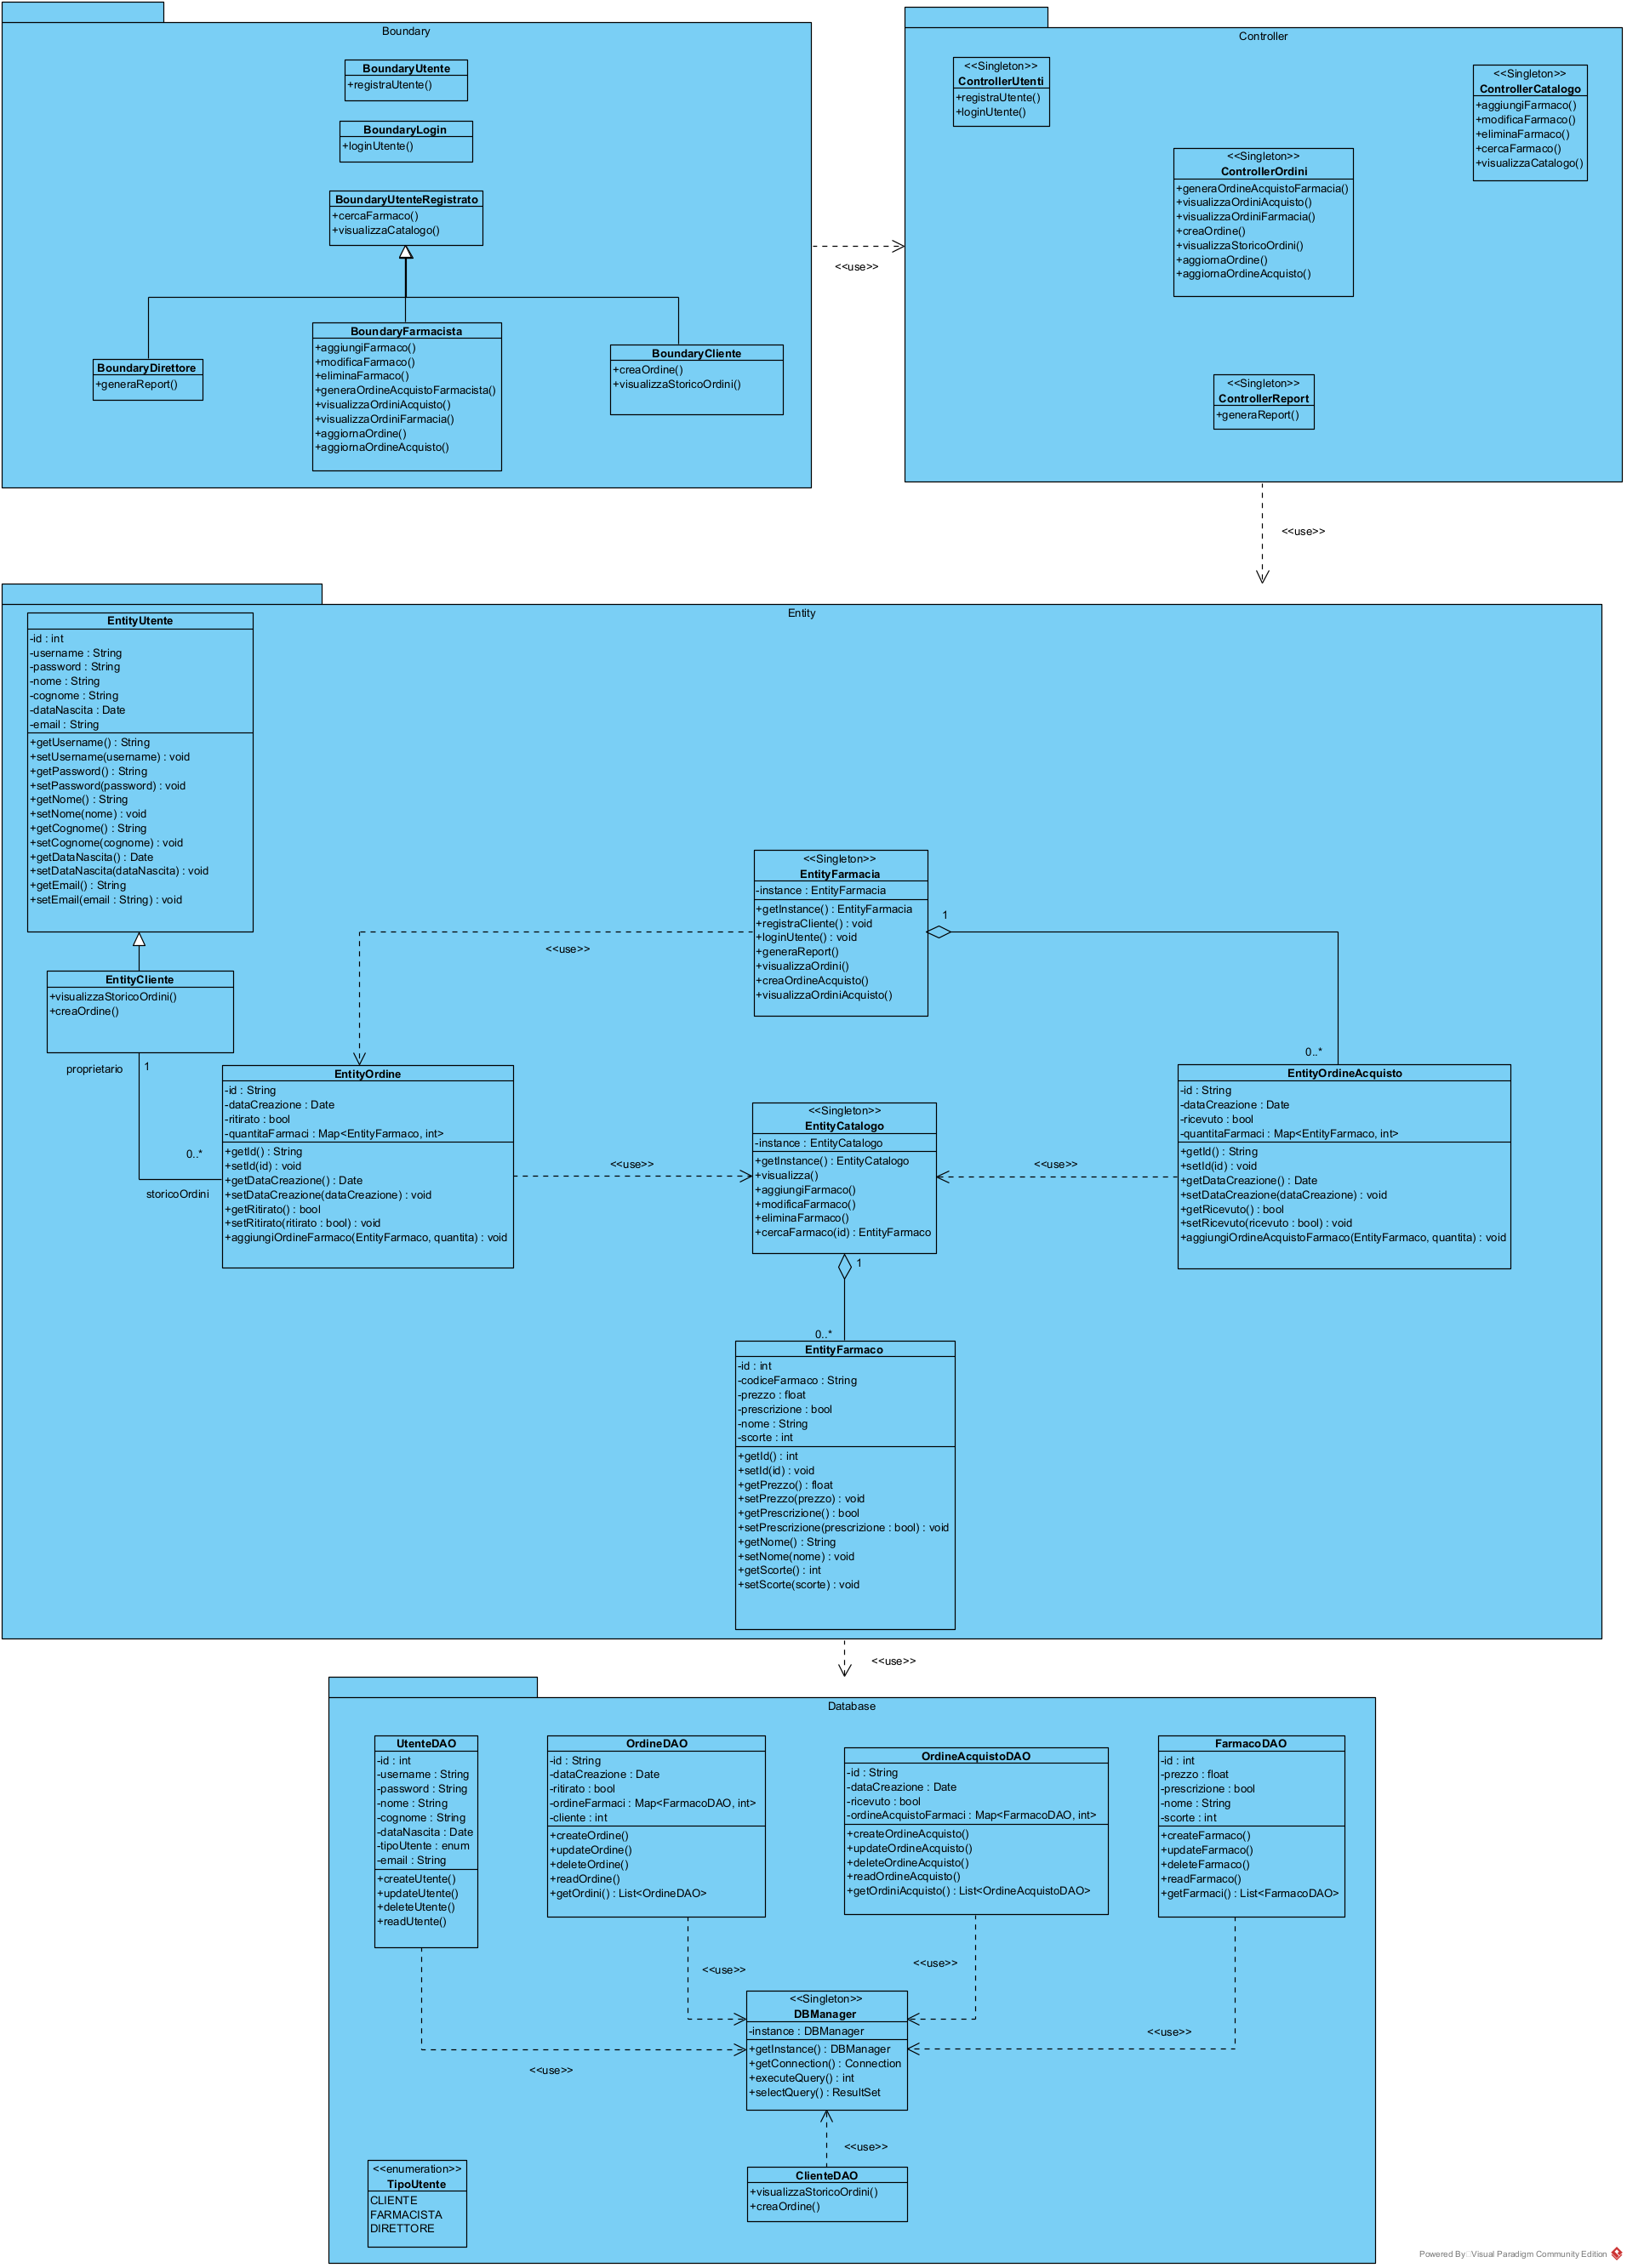
\includegraphics[width=\linewidth]{assets/ClassDiagramProgettazione.png}
    \caption{Diagramma delle classi di progettazione}
\end{figure}

\pagebreak

\section{Modello Entity-Relationship del Database}

\begin{figure}[h]
    \centering
	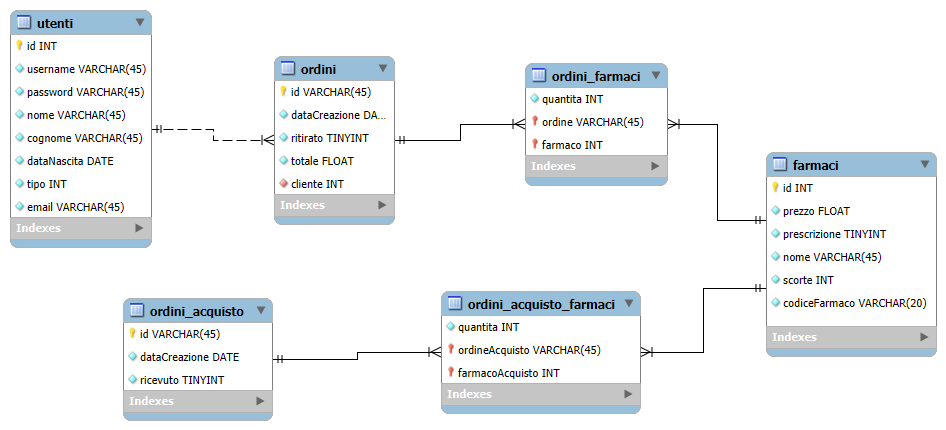
\includegraphics[width=\linewidth]{assets/Modello_ER_DB.png}
    \caption{Modello E/R del Database}
\end{figure}

\section{Diagrammi di sequenza}
\chapter{Implementazione}

\section{Specifiche di implementazione Java}

Riportiamo di seguito le classi Java utilizzate, con la loro suddivisione in package:

\begin{itemize}
	\item \textbf{Package farmacia.boundary}
	\begin{itemize}
		\item RegisterPage
		\item LoginPage
		\item HomePageCliente
		\item VisualizzaCatalogoPage
		\item FarmaciTableModel
		\item CreaOrdinePage
		\item VisualizzaStoricoOrdiniPage
		\item CercaFarmacoPage
		\item HomePageFarmacista
		\item AggiungiFarmacoPage
		\item EliminaFarmacoPage
		\item VisualizzaCatalogoFarmacistaPage
		\item VisualizzaOrdiniClientiPage
		\item VisualizzaOrdiniAcquistoPage
		\item GeneraOrdineAcquistoPage
		\item ScegliFarmacoModificaPage
		\item RegistraRitiroOrdineClientePage
		\item RegistraConsegnaOrdineAcquistoPage
		\item HomePageDirettore
		\item GeneraReportPage
	\end{itemize}
	\item \textbf{Package farmacia.boundary.creaordine}
	\begin{itemize}
		\item CreaOrdinePage
		\item OrdineTableModel
		\item OrdineTableColumnModel
		\item QuantitaCellEditor
	\end{itemize}
	\item \textbf{Package farmacia.boundary.datepicker}
	\begin{itemize}
		\item DatePanel
		\item DateTextField
	\end{itemize}
	\item \textbf{Package farmacia.controller}
	\begin{itemize}
		\item ControllerCatalogo
		\item ControllerOrdini
		\item ControllerUtenti
		\item ControllerReport
	\end{itemize}
	\item \textbf{Package farmacia.entity}
	\begin{itemize}
		\item EntityCatalogo
		\item EntityCliente
		\item EntityUtente
		\item EntityFarmacia
		\item EntityFarmaco
		\item EntityOrdine
		\item EntityOrdineAcquisto
		\item Sessione
	\end{itemize}
	\item \textbf{Package farmacia.database}
	\begin{itemize}
		\item DBManager
		\item UtenteDAO
		\item FarmacoDAO
		\item OrdineDAO
		\item OrdineAcquistoDAO
	\end{itemize}
	\item \textbf{Package farmacia.dto}
	\begin{itemize}
		\item DTO
	\end{itemize}
	\item \textbf{Package farmacia.exceptions}
	\begin{itemize}
		\item DBException
		\item LoginFailedException
		\item RegistrationFailedException
		\item FarmacoCreationFailedException
		\item FarmacoNotFoundException
		\item OrderCreationFailedException
		\item OrderNotFoundException
		\item ReportException
	\end{itemize}
	\item \textbf{Package farmacia.test.controllercatalogo}
	\begin{itemize}
		\item AggiungiFarmacoTest
		\item CercaFarmacoTest
		\item CercaFarmacoInesistenteTest
		\item EliminaFarmacoTest
		\item ModificaFarmacoTest
		\item ModificaFarmacoInesistenteTest
	\end{itemize}
	\item \textbf{Package farmacia.test.controllerutenti}
	\begin{itemize}
		\item LoginUtenteTest
		\item RegistraUtenteTest
	\end{itemize}
	\item \textbf{Package farmacia.test.controllerordini}
	\begin{itemize}
		\item CreaOrdineTest
		\item VisualizzaStoricoOrdiniTest
		\item AggiornaOrdineTest
		\item AggiornaOrdineAcquistoFarmaciaTest
		\item GeneraOrdineAcquistoFarmacistaTest
	\end{itemize}
	\item \textbf{Package farmacia.testcontrollerreport}
	\begin{itemize}
		\item GeneraReportTest
	\end{itemize}
	\item \textbf{Package farmacia.util}
	\begin{itemize}
		\item Utility
		\item TipoUtente
	\end{itemize}
	\item \textbf{Package farmacia}
	\begin{itemize}
		\item Main
	\end{itemize}
\end{itemize}

\chapter{Testing}

\section{Test strutturale}

\subsection{\texttt{creaOrdine()}}

\paragraph{Codice Java}

\inputminted[breaklines,tabsize=4,linenos]{java}{chapters/testing_white_box/creaOrdine.java}

\vfill

\pagebreak

\paragraph{Control Flow Graph}\mbox{}\newline

\noindent\begin{minipage}[t]{0.58\linewidth}
	\vspace{0pt}
	Il numero di cammini linearmente indipendenti è detto \emph{numero ciclomatico} di McCabe, e può essere calcolato equivalentemente in uno dei modi seguenti. Sia $G$ il grafo della funzione, allora risulta:
	\begin{enumerate}
		\item $V(G) = E - N + 2$ in cui $E = \text{\#archi in } G$, $N = \text{\#nodi in } G$
		\item $V(G) = P + 1$ con $P = \text{\#predicati in } G$
		\item $V(G) = R + 1$ con $R = \text{\#regioni chiuse in } G$
	\end{enumerate}%
	Nel nostro caso:%
	\begin{itemize}
		\item $E = 16$
		\item $N = 12$
		\item $P = 5$
		\item $R = 5$
	\end{itemize}%
	\begin{enumerate}
		\item $V(G) = E - N + 2 = 16 - 12 + 2 = 6$
		\item $P + 1 = 5 + 1 = 6$
		\item $R + 1 = 5 + 1 = 6$
	\end{enumerate}%
	\noindent I cammini di base sono:
	\begin{enumerate}
		\item 0-1
		\item 0-2
		\item 0-2-3-4-9-11
		\item 0-2-3-4-9-10-11
		\item 0-2-3-4-5-6-8-4-9-11
		\item 0-2-3-4-5-6-7-8-4-9-10-11
	\end{enumerate}
\end{minipage}
\hfill
\noindent\begin{minipage}[t]{0.38\linewidth}
	\vspace{0pt}
	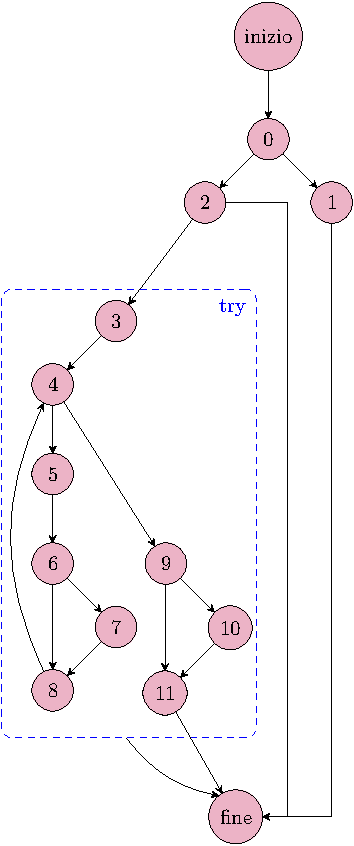
\includegraphics{chapters/testing_white_box/cfg_creaOrdine.pdf}
\end{minipage}

\vfill
\pagebreak

\paragraph{Test suite strutturale}\mbox{}\newline

\begin{table}[!hbp]
	\centering
	\begin{scenery}{colspec=lX}
		Caso d'uso: & CreaOrdine \\
		Attore primario & Cliente \\
		Attore secondario & - \\
		Descrizione & Un cliente genera un ordine contenente farmaci presenti in catalogo \\
		Pre-condizioni & Il cliente è autenticato \\
		{Sequenza di eventi \\ principale} &
			\begin{enumerate}
				\item Il cliente richiede al sistema di creare un ordine
				\item Il sistema mostra a video la lista dei farmaci
				\item Finché il cliente vuole aggiungere farmaci all'ordine
				\begin{enumerate}[label*=\arabic*.]
					\item Se viene richiesto un farmaco non da banco, il sistema chiede conferma del possesso della prescrizione
					\item Il cliente seleziona la quantità di farmaco desiderata
					\item Il sistema verifica che le scorte siano sufficienti
					\item Il sistema crea l'ordine con i farmaci inseriti e aggiorna le scorte
					\item \textit{punto di estensione}: GeneraOrdineAcquisto
				\end{enumerate}
				\item Il sistema mostra al cliente il resoconto dell'ordine e l'importo totale
				\item Se il cliente conferma l'acquisto
				\begin{enumerate}[label*=\arabic*.]
					\item Il sistema restituisce una ricevuta al cliente
				\end{enumerate}
				\item Altrimenti
				\begin{enumerate}[label*=\arabic*.]
					\item Il sistema elimina l'ordine
				\end{enumerate}
			\end{enumerate} \\
		Post-condizioni & È stato correttamente generato un ordine \\
		Casi d'uso correlati & Nessuno \\
		{Sequenza di eventi \\ alternativa} &
			\begin{enumerate}
				\item Al punto 3.1, il sistema mostra un messaggio di errore se il cliente non è in possesso della prescrizione
				\begin{enumerate}[label*=\arabic*.]
					\item Il farmaco non viene aggiunto all'ordine, il caso d'uso prosegue al punto 3
				\end{enumerate}
				\item Al punto 3.3, il sistema rileva che le scorte non sono sufficienti
					\begin{enumerate}[label*=\arabic*.]
						\item Il farmaco viene rimosso dall'ordine
					\end{enumerate}
			\end{enumerate} \\
	\end{scenery}
\end{table}


\vfill
\pagebreak

\subsection{\texttt{modificaFarmaco()}}

\paragraph{Codice Java}

\inputminted[breaklines,tabsize=4,linenos]{java}{chapters/testing_white_box/modificaFarmaco.java}

\paragraph{Control Flow Graph}\mbox{}\newline

\noindent\begin{minipage}[t]{0.58\linewidth}
	\vspace{0pt}
	Il numero di cammini linearmente indipendenti è detto \emph{numero ciclomatico} di McCabe, e può essere calcolato equivalentemente in uno dei modi seguenti. Sia $G$ il grafo della funzione, allora risulta:
	\begin{enumerate}
		\item $V(G) = E - N + 2$ in cui $E = \text{\#archi in } G$, $N = \text{\#nodi in } G$
		\item $V(G) = P + 1$ con $P = \text{\#predicati in } G$
		\item $V(G) = R + 1$ con $R = \text{\#regioni chiuse in } G$
	\end{enumerate}%
	Nel nostro caso:%
	\begin{itemize}
		\item $E = 6$
		\item $N = 5$
		\item $P = 2$
		\item $R = 2$
	\end{itemize}%
	\begin{enumerate}
		\item $V(G) = E - N + 2 = 6 - 5 + 2 = 3$
		\item $P + 1 = 2 + 1 = 3$
		\item $R + 1 = 2 + 1 = 3$
	\end{enumerate}%
	\noindent I cammini di base sono:
	\begin{enumerate}
		\item 0-1
		\item 0-1-2-4-1
		\item 0-1-2-3-4-1
	\end{enumerate}
\end{minipage}
\hfill
\noindent\begin{minipage}[t]{0.38\linewidth}
	\vspace{0pt}
	\begin{tikzpicture}[
    node/.style={circle, minimum height=20pt,text centered, draw=black, fill=purple!30},
    try/.style={rectangle, rounded corners=5, dashed, inner sep=8pt, draw=blue},
    node distance=0.8cm,
    arrow/.style={->,>=stealth}
]
\node (start) [node] {inizio};
\node (0) [node, below=of start] {$0$};
\node (1) [node, below=of 0] {$1$};
\node (2) [node, below left=of 1] {$2$};
\node (3) [node, below left=of 2] {$3$};
\node (4) [node, below=1.5cm of 2] {$4$};
\node (fine) [node, below = 4cm of 1] {fine};
\node (try) [try, fit=(0) (1) (2) (3) (4)] {};
\node [anchor=north west, inner sep=5pt, text=blue] at (try.north west) {try};



\draw[arrow] (start) -- (0);
\draw[arrow] (0) -- (1);
\draw[arrow] (1) -- (2);
\draw[arrow] (2) -- (3);
\draw[arrow] (2) -- (4);
\draw[arrow] (2) -- (4);
\draw[arrow] (3) -- (4);
\draw[arrow] (4) to [bend right=10] (1);
\draw[arrow] (1) to [bend left=50] (fine);
\draw[arrow] (try) to [bend right=10] (fine) {};

\end{tikzpicture}
\end{minipage}

\vfill
\pagebreak

\paragraph{Test suite strutturale}\mbox{}\newline

\begin{table}[!hbp]
	\centering
	\footnotesize
	\begin{tblr}{
			colspec = lXXXXX,
			hlines, vlines,
			row{1} = {font=\bfseries},
			measure=vbox
		}
		{Test \\ Case \\ ID} & Descrizione & {Cammino \\ Coperto} & Pre-condizioni & Input & Esito \\
		1 & Il farmaco è presente nel DB ma non nella collection locale, che risulta vuota & 0-1 & Il farmaco è presente nel DB ma non nella collection locale & -- &
       	Cammino non percorribile: la collection locale è sempre sincronizzata con il DB \\
		2 & La collection locale ha un solo farmaco che non è quello da modificare & 0-1-2-4-1 & -- & -- & Cammino non percorribile: se il farmaco è presente nel DB, deve essere presente anche nella collection locale \\
		3 & Il farmaco esiste & 0-1-2-3-4-1 & Il farmaco esiste & {Nome: Plasil \\ Prezzo: 11.50 \euro \\ Scorte: 30 \\ Prescrizione: \texttt{True}} & Farmaco modificato \\
	\end{tblr}
\end{table}


\section{Test funzionale}
In questa sezione ci occupiamo di riportare i risultati associati alla test suite definita nel \hyperref[cap:piano_test_funzionale]{Capitolo 4}. Di seguito sono riportati gli esiti dell'esecuzione dei vari test case sull'implementazione Java del servizio richiesto: in particolare non vengono mostrati i casi di test basati esclusivamente sull'input validation, effettuata completamente a livello \texttt{Boundary}. I test riportati, dunque, sono eseguiti a livello \texttt{Controller}.

I test sono stati implementati utilizzando il framework \texttt{JUnit}. Per la corretta esecuzione dei test è necessario eseguire nel pannello di controllo dell'istanza \texttt{MySQL} lo script \texttt{svuota\_db\_pre\_test.sql}, che svuota tutte le tabelle del database nell'ordine corretto (per rispettare i vincoli inter-relazionali), oltre a registrare un account da farmacista ed uno da direttore. È necessario, inoltre, disabilitare la \texttt{SAFE UPDATE/DELETE MODE} di \texttt{MySQL}.

\subsection{RegistraCliente}

\begin{table}[!hb]
	\centering
	\footnotesize
	\begin{testsuite}{colspec = lXXllXXl}
		{Test \\ Case \\ ID} & Descrizione & Classi di Equivalenza Coperte & {Pre-\\condizioni} & Input & {Output \\ Attesi} & {Post-condizioni \\ Attese} & Esito\\
		1 & Tutti gli input validi & Nome, Cognome, Username, Password, Email, DataNascita validi & {Il cliente non \\ è ancora \\ registrato \\ nel sistema} & {Nome: Mario \\ Cognome: Rossi \\ Username: mariorossi \\ Password: miapassword \\ Email: mario@gmail.com \\ DataNascita: 22-06-1989} & Registrazione effettuata & Il cliente è stato correttamente registrato nel sistema & \texttt{PASS} \\
		13 & Username già presente nel sistema & Username già esistente \texttt{[ERROR]}, Nome, Cognome, Password, DataNascita ed Email validi & {Username \\ ``pippo2002'' \\ già presente \\ nel sistema} & {Nome: Pippo \\ Cognome: Baudo \\ Username: pippo2002 \\ Password: miapassword \\ Email: pippo@gmail.com \\ DataNascita: 1989-06-22} & {Username già \\ utilizzato} & -- & \texttt{PASS} \\
		14 & Email già presente nel sistema & Email già esistente \texttt{[ERROR]}, Nome, Cognome, Password, DataNascita e Username validi & {Email ``pippo@-\\gmail.com'' \\ già presente \\ nel sistema} & {Nome: Pippo \\ Cognome: Baudo \\ Username: pippo2002 \\ Password: miapassword \\ Email: pippo@gmail.com \\ DataNascita: 1989-06-22} & {Email già \\ utilizzata} & -- & \texttt{PASS} \\
	\end{testsuite}
\end{table}

\subsection{LoginUtente}

\begin{table}[H]
	\centering
	\footnotesize
	\begin{testsuite}{colspec = lXXXXXXl}
		{Test \\ Case \\ ID} & Descrizione & Classi di Equivalenza Coperte & Pre-condizioni & Input & {Output \\ Attesi} & {Post-condizioni \\ Attese} & Esito \\
		1 & Tutti gli input validi & Username, Password validi & {L'utente deve essere \\ correttamente \\ registrato nel sistema} & {Username: mariorossi \\ Password: miapassword} & Login effettuato & L'utente è entrato correttamente nel sistema & \texttt{PASS}\\
		6 & Password errata & Password errata \texttt{[ERROR]}, Username valido & L'utente esiste nel sistema e ha come password `passwd' & {Username: mariorossi \\ Password: ciao} & Password errata & -- & \texttt{PASS}\\
		7 & Username non registrato & Username non registrato \texttt{[ERROR]} & L'utente non esiste nel sistema & {Username: geronimo \\ Password: stilton} & Utente non registrato & -- & \texttt{PASS}\\
	\end{testsuite}
\end{table}

\subsection{AggiungiFarmaco}

\begin{table}[H]
	\centering
	\footnotesize
	\begin{testsuite}{colspec = lXXXlXXl}
		{Test \\ Case \\ ID} & Descrizione & Classi di Equivalenza Coperte & Pre-condizioni & Input & {Output \\ Attesi} & {Post-condizioni \\ Attese} & Esito \\
		1 & Tutti gli input validi & Nome, Prezzo, Scorte e Prescrizione (sia \texttt{True} che \texttt{False}) validi & Il farmaco non è presente nel sistema & {Nome: Rocefin \\ Prezzo: 15.00 \euro \\ Scorte: 60 \\ Prescrizione: \texttt{boolean}} & Farmaco aggiunto & Il farmaco viene correttamente aggiunto al catalogo & \texttt{FAIL} \\
		6 & Nome già memorizzato & Nome già memorizzato \texttt{[ERROR]}, Prezzo, Scorte e Prescrizione (sia \texttt{True} che \texttt{False}) validi & Esiste già un farmaco con il nome inserito & {Nome: Cistalgan \\ Prezzo: 19.90 \euro \\ Scorte: 50 \\ Prescrizione : \texttt{boolean}} & Farmaco già esistente & -- & \texttt{PASS} \\
	\end{testsuite}
\end{table}
Il test case 1 per la funzionalità AggiungiFarmaco ha dato come esito \texttt{FAIL}, generando un'eccezione a livello database. Abbiamo riscontrato la causa del malfunzionamento nel seguente snippet di codice presente nella classe \texttt{FarmacoDAO}:
\begin{minted}[breaklines,tabsize=4,linenos]{java}
String query = String.format("INSERT INTO farmaci (prezzo, prescrizione, nome, scorte, codice) " + "VALUES (%.2f, %d, '%s', %d, '%s');",
			this.prezzo, this.prescrizione ? 1 : 0, this.nome, this.scorte, this.codice
		);
\end{minted}
Il problema è stato individuato a livello del metodo \texttt{String.format(...)}, che stampa le variabili \texttt{float} utilizzando la virgola come separatore tra parte intera e parte decimale (per la convenzione geografica), dunque qualsiasi numero decimale passato nel parametro \texttt{prezzo} viene diviso, a livello \texttt{SQL}, in due parametri. Il corpo della chiamata è stato modificato come segue:
\begin{minted}[breaklines,tabsize=4,linenos]{java}
String query = String.format(Locale.US, "INSERT INTO farmaci (prezzo, prescrizione, nome, scorte, codice) " + "VALUES (%.2f, %d, '%s', %d, '%s');",
			this.prezzo, this.prescrizione ? 1 : 0, this.nome, this.scorte, this.codice
		);
\end{minted}
Tale problematica è presente in ogni metodo delle classi \texttt{DAO} che esegue query \texttt{SQL} contenenti un parametro di tipo \texttt{float}. La documentazione di \texttt{java.util.String} riporta che è possibile forzare la rappresentazione geografica dei numeri floating point utilizzando la costante \texttt{Locale.US}: con questo accorgimento, tutti i test che presentano questa problematica restituiscono esito positivo.

\subsection{CercaFarmaco}

\begin{table}[H]
	\centering
	\footnotesize
	\begin{testsuite}{colspec = lXXXlXll}
		{Test \\ Case \\ ID} & Descrizione & Classi di Equivalenza Coperte & Pre-condizioni & Input & {Output \\ Attesi} & {Post-\\condizioni \\ Attese} & Esito \\
		1 & Nome del farmaco valido & Nome del farmaco valido & Il farmaco è presente nel catalogo & Nome: Tachipirina & Il farmaco viene mostrato a video & -- & \texttt{PASS} \\
		4 & Nome di un farmaco che non esiste & Nome di un farmaco che non esiste \texttt{[ERROR]} & Il farmaco con nome ``Tachipirina'' non esiste & Nome: Tachipirina & Il farmaco non esiste & -- & \texttt{PASS} \\
	\end{testsuite}
\end{table}

\subsection{EliminaFarmaco}

\begin{table}[H]
	\centering
	\footnotesize
	\begin{testsuite}{colspec = lXXXlXXl}
		{Test \\ Case \\ ID} & Descrizione & Classi di Equivalenza Coperte & Pre-condizioni & Input & {Output \\ Attesi} & {Post-condizioni \\ Attese} & Esito \\
		1 & Nome del farmaco valido & Nome del farmaco valido & Il farmaco è presente nel catalogo & Nome: Tachipirina & Farmaco cancellato & Il farmaco viene cancellato dal catalogo & \texttt{PASS} \\
		4 & Il farmaco non esiste & Farmaco non presente nel sistema \texttt{[ERROR]} & Non esiste il farmaco chiamato ``Tachipirina'' & Nome: Tachipirina & Non puoi eliminare un farmaco che non esiste & -- & \texttt{PASS} \\
	\end{testsuite}
\end{table}

\subsection{ModificaFarmaco}

\begin{table}[H]
	\centering
	\footnotesize
	\begin{testsuite}{colspec = lXXXlXXl}
		{Test \\ Case \\ ID} & Descrizione & Classi di Equivalenza Coperte & Pre-condizioni & Input & {Output \\ Attesi} & {Post-condizioni \\ Attese} & Esito \\
		1 & Tutti gli input validi, prescrizione \texttt{True} & Nome, Prezzo, Scorte e Prescrizione (\texttt{True}) validi & Il farmaco è presente nel sistema & {Nome: Tachipirina \\ Prezzo: 11.44 \euro \\ Scorte: 100 \\ Prescrizione: \texttt{True}} & {Modifica \\ effettuata} & Il farmaco viene correttamente modificato & \texttt{PASS} \\
		2 & Tutti gli input validi, prescrizione \texttt{False} & Nome, Prezzo, Scorte e Prescrizione (\texttt{False}) validi & Il farmaco è presente nel sistema & {Nome: Tachipirina \\ Prezzo: 11.44 \euro \\ Scorte: 100 \\ Prescrizione: \texttt{False}} & {Modifica \\ effettuata} & Il farmaco viene correttamente modificato & \texttt{PASS} \\
		7 & Il nome del farmaco non esiste & Nome non presente nel sistema \texttt{[ERROR]}, Prezzo, Scorte e Prescrizione validi & Il farmaco ``Tachipirina'' non esiste nel sistema & {Nome: Tachipirina \\ Prezzo: 11.44 \euro \\ Scorte: 100 \\ Prescrizione: \texttt{False}} & Il farmaco non esiste & -- & \texttt{PASS} \\
	\end{testsuite}
\end{table}

\subsection{GeneraReport}

\begin{table}[H]
	\centering
	\footnotesize
	\begin{testsuite}{colspec = llXXXl}
		{Test \\ Case \\ ID} & Descrizione & {Classi di Equivalenza \\ Coperte} & Input & Output Attesi & Esito \\
		1 & {Tutti gli input \\ validi} & DataInizio, DataFine validi & {DataInizio: 01-06-2024 \\ DataFine: 31-06-2024} & Il report viene generato & \texttt{PASS} \\
	\end{testsuite}
\end{table}

\subsection{GeneraOrdineAcquistoFarmacista}

\begin{table}[H]
	\centering
	\footnotesize
	\begin{testsuite}{colspec = lXXXlXXl}
		{Test \\ Case \\ ID} & Descrizione & Classi di Equivalenza Coperte & Pre-condizioni & Input & {Output \\ Attesi} & {Post-condizioni \\ Attese} & Esito \\
		1 & Ordine valido & Farmaci-Quantità valido & Esistono nel sistema i farmaci 'Tachipirina' e 'Fluifort' & {[('Tachipirina', 5),\\ ('Fluifort', 10)]} & Ordine di acquisto generato & Un ordine di acquisto viene correttamente creato & \texttt{PASS} \\
		2 & Ordine vuoto & Lista vuota \texttt{[ERROR]} & -- & -- & Non puoi creare un ordine di acquisto vuoto & -- & \texttt{PASS} \\
	\end{testsuite}
\end{table}

\subsection{RitiraOrdine}

\begin{table}[H]
	\centering
	\footnotesize
	\begin{testsuite}{colspec = lXXXXXXl}
		{Test \\ Case \\ ID} & Descrizione & Classi di Equivalenza Coperte & Pre-condizioni & Input & {Output \\ Attesi} & {Post-condizioni \\ Attese} & Esito \\
		1 & Id dell'ordine valido & Id dell'ordine valido & -- & Id: 5ea930bc-f0a5-427a-8ca1-f9a2a6146948 & Stato ordine cambiato con successo & Lo stato dell'ordine è stato cambiato con successo & \texttt{PASS} \\
		4 & Id inesistente & Id inesistente \texttt{[ERROR]} & Non esiste un farmaco con id ``5ea930bc-f0a5-427a-8ca1-f9a2a6146948'' & Id: 5ea930bc-f0a5-427a-8ca1-f9a2a6146948 & L'ordine non esiste & -- & \texttt{PASS} \\
	\end{testsuite}
\end{table}

\subsection{RegistraConsegnaOrdineAcquisto}

\begin{table}[H]
	\centering
	\footnotesize
	\begin{testsuite}{colspec = lXXXXXXl}
		{Test \\ Case \\ ID} & Descrizione & Classi di Equivalenza Coperte & Pre-condizioni & Input & {Output \\ Attesi} & {Post-condizioni \\ Attese} & Esito \\
		1 & Id dell'ordine di acquisto valido & Id dell'ordine di acquisto valido & -- & {Id: 5ea930bc-f0a5-427a-8ca1-f9a2a6146948} & Ordine ricevuto & Lo stato dell'ordine di acquisto e le scorte in magazzino sono aggiornati & \texttt{PASS} \\
		4 & Id inesistente & Id inesistente \texttt{[ERROR]} & Non esiste un ordine di acquisto con Id ``5ea930bc-f0a5-427a-8ca1-f9a2a6146948'' & Id: 5ea930bc-f0a5-427a-8ca1-f9a2a6146948 & L'ordine di acquisto non esiste & -- & \texttt{PASS} \\
	\end{testsuite}
\end{table}

\subsection{CreaOrdine}

\begin{table}[H]
	\centering
	\footnotesize
	\begin{testsuite}{colspec = lXXXlXXl}
		{Test \\ Case \\ ID} & Descrizione & Classi di Equivalenza Coperte & Pre-condizioni & Input & {Output \\ Attesi} & {Post-condizioni \\ Attese} & Esito \\
		1 & Ordine valido, l'ordine non esaurisce le scorte di nessun farmaco & Farmaci-Quantità valido & Esistono nel sistema i farmaci 'Tachipirina' e 'Fluifort' con scorte rispettivamente di 80 e 120 & {[('Tachipirina', 5),\\ ('Fluifort', 10)]} & Ordine generato & Ordine creato: scorte in magazzino decrementate & \texttt{PASS} \\
		2 & Ordine valido, l'ordine esaurisce le scorte di un farmaco & Farmaci-Quantità valido & Esistono nel sistema i farmaci 'Tachipirina' e 'Fluifort' con scorte rispettivamente di 80 e 120 & {[('Tachipirina', 80),\\ ('Fluifort', 10)]} & Ordine generato & Ordine creato. Le scorte in magazzino vengono correttamente decrementate e viene generato un ordine di fornitura per il farmaco esaurito, richiedendone una quantità di default & \texttt{PASS} \\
		3 & Ordine invalido per scorte insufficienti & Scorte insufficienti \texttt{[ERROR]} & Esistono nel sistema i farmaci 'Tachipirina' e 'Fluifort' con scorte rispettivamente di 80 e 120 & {[('Tachipirina', 5),\\ ('Fluifort', 150)]} & Ordine non creato per scorte insufficienti & -- & \texttt{PASS} \\
		4 & Ordine vuoto & Lista vuota \texttt{[ERROR]} & -- & -- & Non puoi creare un ordine vuoto & -- & \texttt{PASS} \\
	\end{testsuite}
\end{table}


\end{document}